\RequirePackage[l2tabu, orthodox]{nag}
\documentclass[12pt]{article}
\usepackage[utf8]{inputenc}
\usepackage[T1]{fontenc}
\usepackage{amsmath, amssymb, amsfonts}
\usepackage{newtxtext, newtxmath}
\usepackage{graphicx}
\usepackage{float}
\usepackage[justification=justified]{caption}
\usepackage{subcaption}
\usepackage{booktabs}
\usepackage{microtype}
\usepackage{setspace}
\usepackage{siunitx}
\usepackage[margin=1in]{geometry}
\usepackage{enumitem}
\usepackage[normalem]{ulem}
\usepackage{rotating}
\usepackage{pdflscape}
\usepackage{multicol}
\usepackage[backgroundcolor=orange, linecolor=black]{todonotes}
\usepackage[overload]{textcase}
\usepackage[autostyle=true, english=american, strict=true]{csquotes}
\usepackage[american]{babel}
\usepackage[colorlinks=true, linktoc=all, linkcolor=magenta, citecolor=black, urlcolor=magenta, breaklinks=true]{hyperref}
\usepackage{cleveref}

\author{Oskar Timo Thoms\thanks{This report builds and expands on the January 2021 report co-authored together with Dane Rowlands and Valerie Percival. The first two sections are edited and expanded versions of the first two sections in the previous report authored by Thoms, Rowlands and Percival, and one of the appendices reproduces the previous report's section on the cross-sectional regression analyses written by Rowlands.}\\Consultant}
\title{Lancet Commission Metrics Working Group:\\Draft Report on Large-N Analyses Extensions}
\date{\today}

\begin{document}

\maketitle
\clearpage
\tableofcontents
\bigskip
\begin{center}
* Starred * section titles indicate substantially new materials not discussed in the previous report.
\end{center}

\clearpage

\section{Introduction}
\label{intro}

Building on earlier work, this draft report summarizes extensions of large-N analyses conducted for the Lancet-SIGHT Commission, whose objective is to examine if and how gender equality and health equity can contribute to more peaceful societies.
The central research question which guides this work is: how does variation in gender equality and health equity (improvements or declines) influence variation in violence and conflict?

The Metrics Working Group explores this question through quantitative analysis of large-N cross-national data, as well as studies based on systematic reviews of the existing literature and the use of descriptive data. To understand the quality of the data for both the large-N and the case studies, we have undertaken a rigorous analysis of indicators used in this research.
Through the analysis of a large number of observations, large-N analysis establishes associations to determine if and how variables relate to each other and if these relationships have statistical significance. Careful statistical analysis can partly account for endogeneity and lessen the chances of spurious associations. Without doing this large-N analysis, we risk making false causal claims about the generalizability of the relationships between gender equality, health equity and peace. In short, large-N analysis can provide greater confidence of the external validity of our analysis.

Inspired by an article by Suri et al (2010), which argues human development and economic growth operate in vicious and virtuous cycles, we decided to test this concept with three variables - health, gender and violence/conflict. Specifically we want to explore:
\begin{itemize}
\item if and how gender inequalities and health inequities and violence reinforce each other in vicious cycles;
\item if and how gender equality, health equity, and peace reinforce each other in virtuous cycles;
\item and if and how interventions to support gender equality and health equity, under the right conditions, have the ability to nudge communities and societies from vicious to virtuous cycles.
\end{itemize}

Our large-N analyses begin to build an evidence base for broad statistical relationships between gender, health, and violence outcomes.
Based on the virtuous and vicious cycles framework proposing that health, gender, and violence variables interact with each other to produce mutually reinforcing negative (vicious) and/or positive (virtuous) patterns, these analyses are guided by the following questions:
\begin{itemize}
\item While accounting for the overall improvements that most countries have experienced in health and gender outcomes in recent decades, do those countries that score low in earlier periods improve less than the global average and/or high performers, or do they perhaps even decline?
\item While accounting for possible ceiling effects, do those countries that score high in earlier periods a) maintain stable and high levels and b) avoid violence?
\item Do countries that experience higher levels of violence a) improve less on gender equality and health outcomes than those with less violence, or b) do their gender and health outcomes perhaps even deteriorate?
\item Are countries that score low on health and gender outcomes more prone to violence than those that score higher?
\end{itemize}

These questions imply considerable complexity, as they examine statistical effects between gender and health outcomes; from gender and health outcomes to violence; and from violence to gender and health outcomes.
Our multivariate regression analyses test these questions in probabilistic terms, not in deterministic fashion.
While there are likely many other important factors influencing health, gender and violence outcomes, we do not develop full causal models of each outcome, but examine whether associations between the three categories of outcomes are consistent with the theoretical framework of virtuous and vicious cycles. We see this as a first useful step in a larger research agenda exploring relationships between health, gender, and peaceful societies.

In the previous report, we examined multivariate models of both cross-sectional and panel data. These two different approaches to modeling cross-national data have complementary advantages and disadvantages.
First, the cross-sectional models allow us to examine long-term changes in outcome variables, over 20-year periods, while the panel models examine short-term variation, from one five-year period to the next but over longer study periods than the cross-sectional analyses.
Second, the two approaches have different methodological trade-offs. While the cross-sectional models make it somewhat easier to address problems of endogeneity and heteroscedasticity, they also have fewer degrees of freedom due to their small sample sizes (i.e. the number of countries included). Panel models are subject to more concerns about endogeneity, heteroscedasticity and serial correlation due to the structure of the data used (several observations of countries over time), but they also have much larger sample sizes allowing for more precision in statistical estimates. We believe that both approaches are valuable in examining the research questions.

In this report, I re-implement and extend the panel analyses to address some questions that emerged in the previous report with respect to the operationalization of vicious and virtuous cycles, the robustness of results, and some differences in findings between the cross-sectional and panel analyses. \Cref{previous} reviews the findings of the previous report, and \Cref{extensions} outlines what extensions are pursued and why. Sections \ref{data} and \ref{methods} discuss the data and methods used, largely repeating the discussion of the previous report and explaining how the classifications are used in the extensions. Sections \ref{results_hg}, \ref{results_violence}, and \ref{discussion} summarize and discuss the results of the new analyses. Finally, \Cref{sequencing} briefly introduces the exploratory work I have done on categorizing the sequencing of change in gender and health outcomes. This work is to be expanded into a pathways typology in the final report.
This draft report is written in such a way that no knowlegde of the previous report is required.
The appendix provides tables summarizing the findings of the main models examined for this report, and reproduces the cross-sectional and panel analyses of the first report for reference.

\section{Findings of the previous report}
\label{previous}

The present report focuses on extensions of the panel analyses, which are in part motivated by some differences in findings between the cross-sectional and panel analyses. In our prior report, the cross-sectional analyses yielded the following conclusions:
\begin{itemize}
\item Over the period from 1995 to 2015 there was a general improvement in the four measures of health and gender used in this analysis.
\item Analyzing performance is complicated due to the presence of ceiling effects. Once a country has obtained a high level of performance in their health and gender performance, the room for additional improvements is quite limited. How we measure improvements is important, as is the manner in which we take into account the limited scope for changes in performance. In the regressions it is generally the case that past good health performance is associated with smaller future improvements, and the same for gender performance measures.
\item In general there is reasonable evidence consistent with the presence of a virtuous feedback loop whereby better past gender performance is associated with improved future health measures, and better past gender measures are associated with improved future health performance.
\item The cross-section variation in health and gender measures is typically well explained by these fairly simple models. The percentage of variation explained by the models (the $R^2$ value) ranges from a low of about 35\% (for the adolescent fertility rate) to over 80\% (for the infant mortality rate).
\item For the most part, the equations also perform well when using only past values of key explanatory variables (no concurrent values). These prediction models are less subject to some of the simultaneity and endogeneity problems with the base equations, and generally still yield comparable $R^2$ values.
\item As is well known from the literature, there is a high degree of inertia in violence on conflict over time. In other words, once countries experience violent conflict, they likely to do so in the future.
\item In the analysis prior conflict is often positively related to future health and gender improvements, which appears to be the consequence of a reduction in past performance and the possibility of recovery. By contrast, and as expected, concurrent (future) violence and conflict is generally negatively related to health and gender improvements.
\item There are many different measures of conflict and violence, and their relationship amongst one another and with health and gender measures is varied and often nuanced. It is difficult to identify one \enquote{summary} and \enquote{best} measure of conflict and violence, or to ascribe one relationship that applies to all of these measures. Investigating the nuances of different violence and conflict measures would be a useful extension of this work.
\item This cross-sectional analysis focuses on three conflict and violence measures (number of years experiencing significant conflict over a period of time, civilian deaths associated with civil conflict, and civilian deaths associated with one-sided violence) all seem to exhibit a negative association with better health and gender measures. More years of female education relative to male appears to have the most consistent negative association with future death and conflict rates. This evidence is supportive of the virtuous/vicious circle proposition, in which better health and gender performance is associated with less violence, which in turn generally contributes to better future health and gender performance.
\end{itemize}

For the interested reader not familiar with the previous report, the cross-sectional analyses and their discussion are reproduced in \Cref{appendix_cs_dane}.

The panel models presented in the previous report led to the following conclusions:

\begin{itemize}
\item As in the cross-sectional analyses, gender and health outcomes are clearly positively correlated with each other. This is consistent with the notion that they reinforce each other.
\item Unlike in the cross-sectional analyses, there is little suggestion of ceiling or convergence effects in these analyses. Better health and gender outcomes in one period are associated with improved outcomes in the next period. This difference between the cross-sectional and panel analyses is likely due to the fact that they are differently structured to examine long-term versus shorter-term associations.
\item While in bivariate associations, poor health and gender outcomes are clearly associated with more violence on average, the role of violence variables in health and gender outcomes is complex, as violence in one period is sometimes associated with better health and gender outcomes in the next period. This result may seem at odds with vicious and virtuous cycles, and points to the need for fuller statistical models based on deeper theoretical work. Moreover, the analyses suggests that different types of violence may matter in different ways.
\item The panel analyses also consider an alternative conceptualization and operationalization of vicious and virtuous cycles, by examining the effects of low and high classifications based on health and gender outcomes. These analyses find clear and consistent support for vicious cycles between health and gender outcomes and in their effects on violence outcomes.
\item While we do not find an analogous result for virtuous cycles, we caution that this may be due to our particular conceptualization, which focuses on the extreme ends of our classifications, i.e. the worst and best performers in comparison to all the countries in between, assuming that virtuous and vicious cycles would be most pronounced in these groups. An extension of this research should examine whether variation in the middle group is consistent with the notion of virtuous cycles. Such research may also advance understanding of pathways of change if it considers sequencing.
\item In models of violence outcomes with interactions between lagged dependent variables with the low and high classifications, we also find strong evidence for three-way vicious cycles, whereby previous violence is associated with renewed (or continued) violence particularly in countries that have very poor health and gender outcomes.
\end{itemize}

The discussion and summary of the panel analyses in the previous report are reproduced in \Cref{appendix_panel}.
We concluded that the findings from the panel analyses suggested more support for vicious than virtuous cycles, particularly between health and gender and in their effects on violence. The evidence varied by measures used and there were many null findings. The effects of violence on gender and health were less clear and often even contradict the theoretical framework. Moreover, the analyses suggested that different types of violence may matter in different ways, pointing to the need for further research into such differences.
% For instance: Why is violence often associated with improved adolescent fertility rates on average?

This research represents useful ground-clearing for further analyses investigating vicious and virtuous cycles between health, gender and violence outcomes. Our previous report argued that these findings warranted further research.
Deeper theoretical work and fuller statistical models are needed to address questions arising from these analyses and explore potential pathways from vicious to virtuous cycles. Such research should account for other possible factors, including, for instance, quality of institutions, inequality, functioning of economies, etc.

We also noted that our analyses were limited in several ways.
First, they examine broad associations and include the same covariates across models.
However, each of the outcome variables may be better modeled with a different set of covariates, based on different scholarly literatures.
Such work may shed light, for instance, on the unexpected association between violence and improved adolescent fertility rates.
Second, the analyses do not examine interactions between different types of violence, or even control for other types of violence in a given model.
Third, the analyses use only the low and high classification to operationalize the vicious and virtuous cycles hypotheses.
However, analyses using a richer classification (including the other groups resulting from our classification procedure) and other interactions may uncover other associations pertaining to vicious and virtuous framework.
% For instance, what are the relative statistical contributions of gender and health outcomes to levels of violence?
Moreover, examining more variation in the classifications could also help with exploring pathways of change. For instance, are there particular sequences of improvements in gender and health outcomes that are more likely to break countries out of vicious cycles?
Another way to explore pathways may be mapping sequences of change in health and gender over decades to determine which pathways are most common or likely to lead to improvements.
% \footnote{In addition, case study analyses of outliers in our models, i.e. countries that defy the general prediction of the models, could be helpful in uncovering pathways of change.}

Despite these limitations, the strong support in particular for vicious cycles between health and gender, and with violence, is convincing and novel.
This result could be further strengthened with robustness checks using other health and gender measures.
It would also be useful to further explore what accounts for differences in findings between the cross-sectional and panel analyses.
While we have noted that the evidence for vicious cycles in the panel analyses may be an artifact of our conceptualization, it is plausible that this result is also due to the different time frames of the analyses. It is possible that virtuous cycles are slow-moving, and thus do not show clear patterns in the panel analyses, while vicious cycles may operate faster.

\section{* Extensions in this report *}
\label{extensions}

In this draft report, I discuss findings from new panel data analyses that address some, though not all, of the limitations noted in the previous section. These analyses extend the previous ones in four different ways.

First, the vicious and virtuous cycles hypothesis can be operationalized in different ways. As noted above, while the cross-sectional analyses examined correlations between the individual gender, health and violence measures, the panel analyses also employ classifications based on health and gender outcomes (see \Cref{data}). To date, however, we only examined the lowest and highest classification groups. The extensions in this report explore variation in the middle by also distinguishing countries which comparatively perform better on gender than on health and vice versa. The objective of this extension is to examine whether vicious and virtuous cycles may be at work across the full range of health and gender outcomes, including in the middle classifications that were previously left out of the analyses. While it makes the analyses more complicated, it also provides interesting new insights.

Second, in the previous report, the panel and cross-national analyses come to some different conclusions, as outlined in \Cref{previous}.\footnote{It is important to note that these differences are largely about the strength and robustness of findings, specifically on virtuous associations, rather than contradictory evidence.}
Further, some members of the Lancet Commission have raised questions about the timeframes required to realize different outcomes. For example, gender equality and virtuous outcomes may take longer to realize change, and thus may only show clear statistical patterns in the cross-sectional analyses and not in the panel analyses because they are structured differently. The extensions address this by considering different timelines in the panel analyses to examine whether this changes the results to more closely match the findings of the cross-sectional analyses. In one set of alternative models, the sample of observations is limited to the period 1995-2015 to match the timeframe of the cross-sectional analyses, and in another set of alternative models, I maintain the timeframe of the panel analyses (1970-2018), but increase the time lag between the independent and dependent variables from five to fifteen years.\footnote{I did not not increase this to twenty years -- the lag used in the cross-sectional analyses -- because the longer the lag, the smaller the sample of observations, thereby affecting statistical precision.} In some cases, considering these different periods or lags leads to more evidence for vicious or virtuous cycles, but in others it weakens the evidence.


Third, the analyses to date find suggestive evidence for vicious cycles between health (measured by life expectancy and infant mortality) and gender (measured by the mean years of schooling ratio of females to males and by the adolescent fertility rate), and with some types of violence. In robustness checks, I examine whether such statistical associations hold for other outcomes, by substituting other health (under-five mortality rate and DALYs) and gender measures (the labour participation ratio of females to males and the Gender Inequality Index) as the dependent variables of the regression analyses. These new measures are chosen based on data availability and to expand the conceptual range of the gender and health dimensions. In preview, the findings of these robustness checks are mixed. Unsurprisingly, the results for the UFMR are very similar to those for the IMR and largely supportive. The models of the labour participation ratio find no evidence of vicious or virtuous cycles, and find some contradictory evidence. The results for DALYs and the Gender Inequality Index provide a mix of supportive and contradictory evidence.

Fourth, the initial analyses strongly suggest that different types of violence -- internal conflict, state repression and societal violence -- may matter in different ways, but these analyses only considered different types of violence separately. Therefore, the extensions include models which also account for other types when examining the role of specific types of violence, to further examine the robustness of findings on vicious and virtuous cycles.\footnote{Other possible approaches are to include aggregate measures, such as deaths from several types of violence, or interactions of different types of violence. Instead,  I choose simple control variables, because aggregate measures are difficult to interpret because they conflate distinct phenomena, and additional interactions would add further complexity to the models.} While the inclusion of these violence variables sometimes weakens the evidence, in many cases, it actually leads to clearer findings on vicious or virtuous cycles.

The remaining sections discuss the data, methods, and findings of the new analyses. Full details of the data preparation and the analyses (including regression details) are available at \href{https://timothoms.github.io/LSC-MWG/}{timothoms.github.io/LSC-MWG/}.

\section{* Data *}
\label{data}

This report uses the same data and panel regression methods as the previous report which it builds on, but altering the research design and models to extend the analyses, as discussed in \Cref{methods}.

Guided by the indicator mapping carried out by the Metrics Working Group, we identified a wide range of health, gender and violence measures as candidates for analyses, and assembled a comprehensive cross-national time-series dataset with the best available data on relevant indicators and key covariates. (A detailed codebook is available at this \href{https://docs.google.com/spreadsheets/d/1KLFTva--XHVBM-IX6qaPtuyzmIlRMnpyjUXfBdJPsag/edit?usp=sharing}{link}.)
Many health and gender measures in particular are subject to many missing data points across countries and over time, and this missingness is unlikely to be random and thus presents a potential threat to inferences. Therefore, based on our evaluation of the quality and coverage of these data, and based on within-category correlations, we chose two representative and commonly accepted variables each for the health (life expectancy and the infant mortality rate) and gender (the ratio of female-to-male mean years of schooling and the age-specific fertility rate for adolescents) dimensions.
To measure violence, we chose several indicators to capture different types, including state-based internal armed conflict, repression and societal violence, and the total and civilian battle-related death rates (per population) resulting from varying types of conflict.
These variables are listed in \Cref{table_vars}.\footnote{The analyses for the previous report included measures of internal war and state torture. This report does not discuss any analyses using these two measures because the results are very similar to those for internal conflict and extra-judicial killings, respectively.}

\begin{table}[!htb]
\centering
\caption{Measures used in the large-N analyses}
\label{table_vars}
\begin{tabular}{llr}
\toprule
Category             & Variable                                                       & Source  \\
\midrule
health               & life expectancy                                                & WPP     \\
health               & \textbf{\textit{infant mortality rate}} (IMR)                  & WPP     \\
health               & \textbf{\textit{under-five mortality rate}} (UFMR)             & WPP     \\
health               & \textbf{\textit{disability-adjusted life years}} (DALYs)       & IHME    \\
gender               & mean years of schooling ratio (MYS)                            & HDR     \\
gender               & \textbf{\textit{adolescent fertility rate}} (AFR)              & WPP     \\
gender               & labour participation ratio                                     & ILO     \\
gender               & Gender Inequality Index (GII)                                  & HDR     \\
state-based conflict & internal conflict incidence                                    & UCDP    \\
state-based conflict & internal war incidence                                         & UCDP    \\
state-based conflict & internal conflict deaths (rate per population)                 & UCDP    \\
state-based conflict & internal conflict civilian deaths (rate per population)        & UCDP    \\
state repression     & one-sided violence (OSV) incidence                             & UCDP    \\
state repression     & one-sided violence (OSV) deaths (rate per population)          & UCDP    \\
state repression     & \textbf{\textit{latent physical integrity measure}}            & Fariss  \\
state repression     & \textbf{\textit{state torture}}                                & V-Dem   \\
state repression     & \textbf{\textit{extra-judicial killings}}                      & V-Dem   \\
societal violence    & non-state conflict (NSC) incidence                             & UCDP    \\
societal violence    & non-state conflict (NSC) deaths (rate per population)          & UCDP    \\
societal violence    & non-state conflict (NSC) civilian deaths (rate per population) & UCDP    \\
societal violence    & homicides (rate per population)                                & ODC/WHO \\
\bottomrule
\end{tabular}
\end{table}


It is important to note that, for easier comparisons of results across variables within each category, we have inverted some variables for the statistical analyses such that higher values of the health and gender variables always indicate \enquote{better} outcomes, while higher values of the violence variables always mean higher levels of violence. The affected variables are indicated by \textbf{\textit{bold italics}} in \Cref{table_vars}. Readers familiar with these measures should keep in mind that this alters how one would usually interpret them.
As data availability and quality generally improves after 1989 and more violence variables exist for this period, the primary period of the analyses is 1989-2018. All variables are aggregated to five-year averages because three of the key health and gender variables are provided as such averages by the World Populations Prospects Database.

For control variables, we use per capita income to represent the level of a country's economic development, and measures of political structure representing the presence or absence of different facets of democracy. While not exhaustive, these variables exhibit useful features in terms of country and year coverage, collection and reporting reliability, and theoretical plausibility.

\begin{table}[!htb]
\centering
\caption{Classification groups used in the analyses extensions}
\label{table_class}
\begin{tabular}{lccccc}
\toprule
                & \multicolumn{5}{l}{\textbf{Gender}} \\
\textbf{Health} & 1st quintile & 2nd quintile & 3rd quintile & 4th quintile & 5th quintile \\
\midrule
1st quintile    & low & low & G>H & G>H & G>H \\
2nd quintile    & low & low & G>H & G>H & G>H \\
3rd quintile    & H>G & H>G & mid & G>H & G>H \\
4th quintile    & H>G & H>G & H>G & upp & upp \\
5th quintile    & H>G & H>G & H>G & upp & upp \\
\bottomrule
\end{tabular}
\end{table}


To help operationalize the vicious and virtuous cycles hypotheses, we developed a classification of countries based on the four health and gender outcomes, creating groups of countries for comparison.
We divided each of the four measures into quintiles at any given point in time and aggregated them along the gender and health dimensions, to produce a 5x5 matrix.
In the analyses for the previous report, we selected the bottom four cells as our low classification and the top four as our high classification. We examined the statistical effects of the lowest and highest classifications, making the assumption that if there are virtuous and vicious cycles present in the data, then they surely would be observed for these two groups. While this expectation was borne out in some models, it also became clear that the large middle category lumped together much potentially interesting variation. Therefore, one of the motivations for the extensions in this report is to explore the possibility that vicious and virtuous cycles may also be at work in the middle. In the analyses in this report, five classification groups are used based on the matrix in \Cref{table_class}: low, mid, upp, and those that score relatively high on health but low on gender ({H>G}), and those that score relatively high on gender but low on health ({G>H}).

\begin{figure}[!htb]
    \centering
    \caption{Life expectancy trends}
    \label{trends_life}
    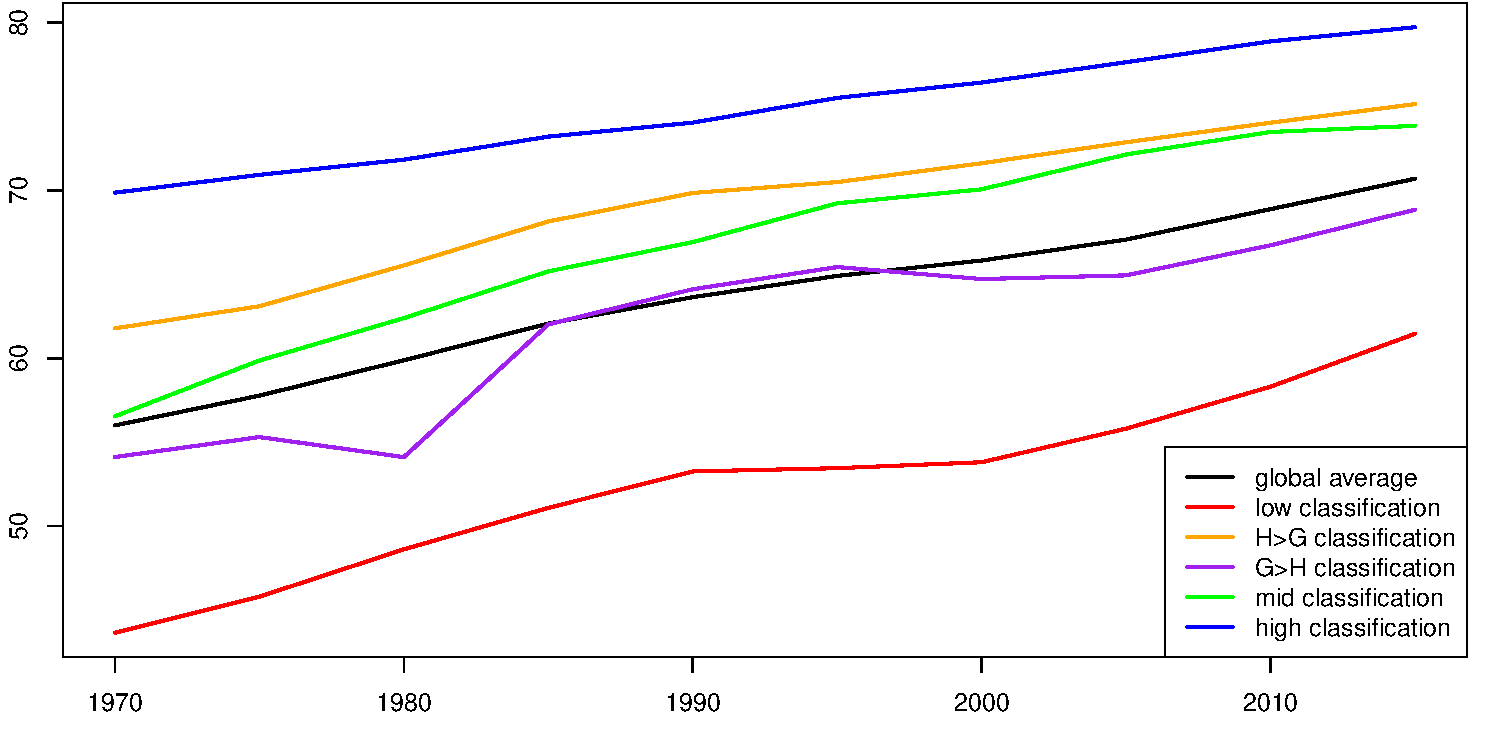
\includegraphics[width=\textwidth]{trend_life_exp_wpp.pdf}
\end{figure}
\begin{figure}[!htb]
    \centering
    \caption{Infant mortality trends}
    \label{trends_imr}
    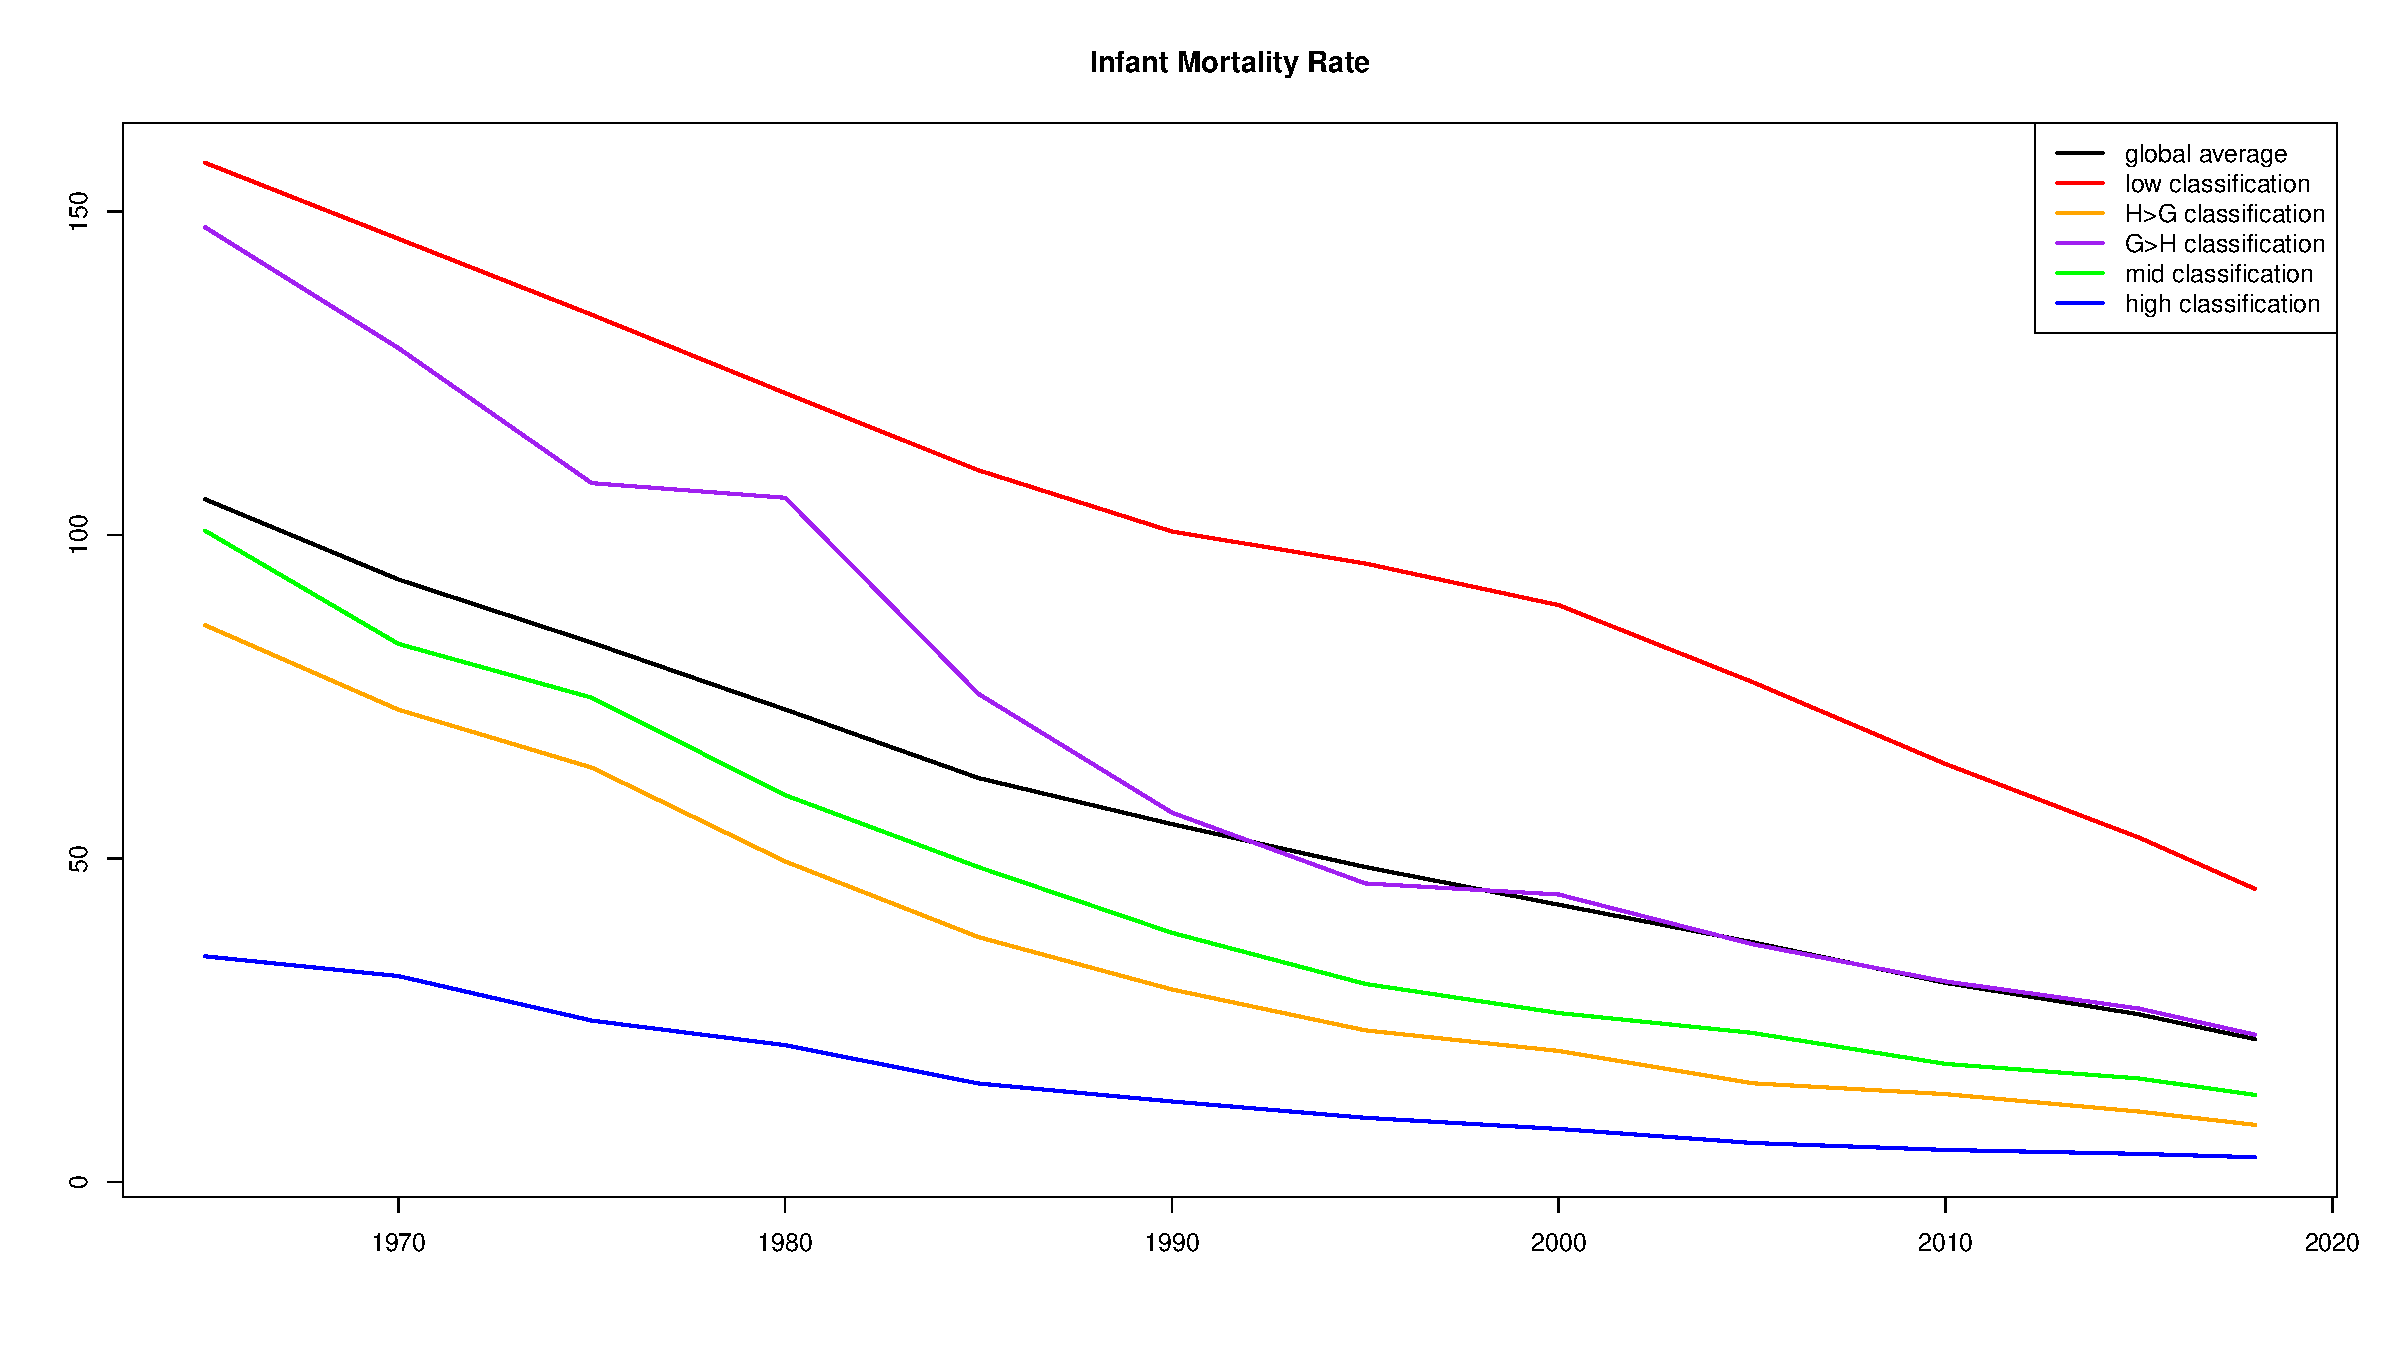
\includegraphics[width=\textwidth]{trend_imr_wpp.pdf}
\end{figure}
\begin{figure}[!htb]
    \centering
    \caption{Mean years of schooling ratio trends}
    \label{trends_mys}
    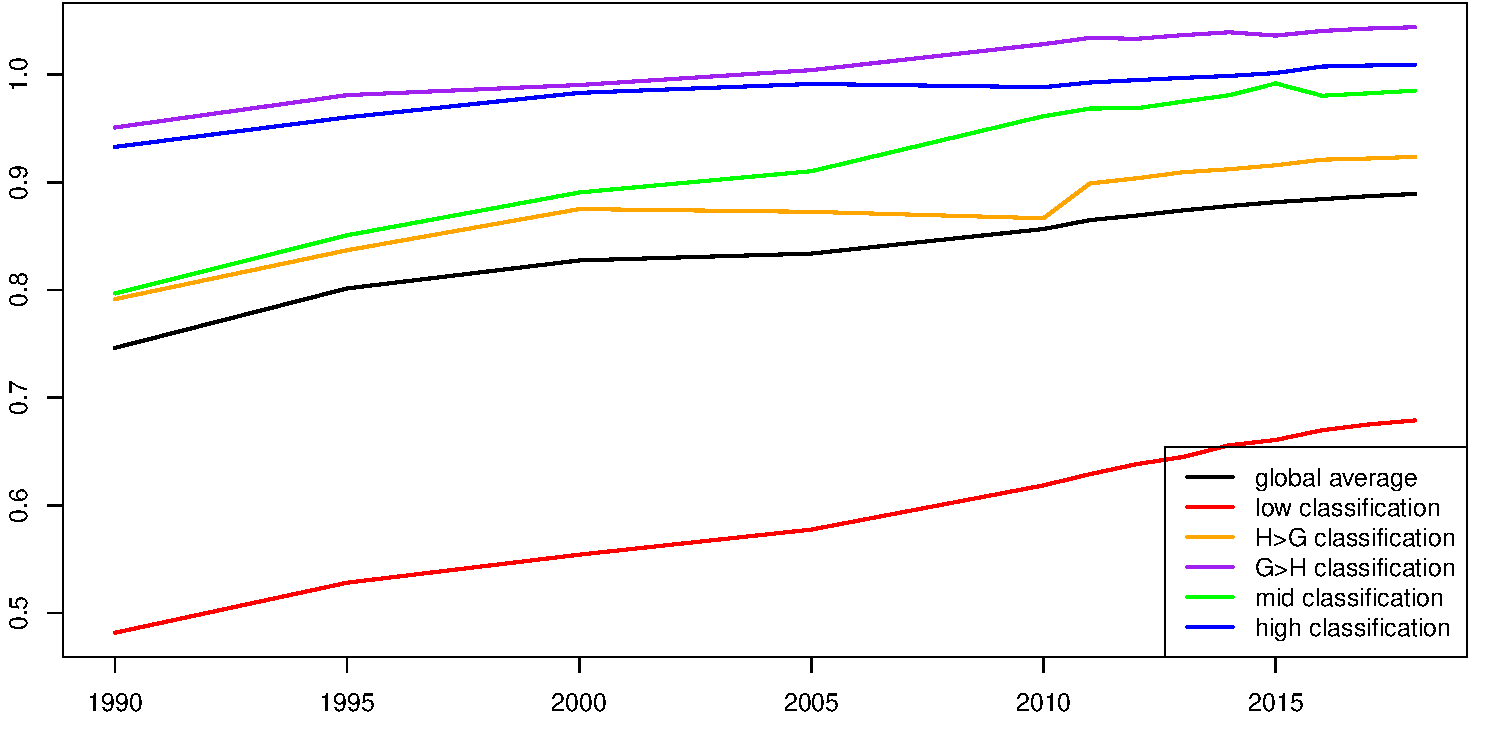
\includegraphics[width=\textwidth]{trend_mys_ratio_hdr.pdf}
\end{figure}
\begin{figure}[!htb]
    \centering
    \caption{Adolescent fertility trends}
    \label{trends_afr}
    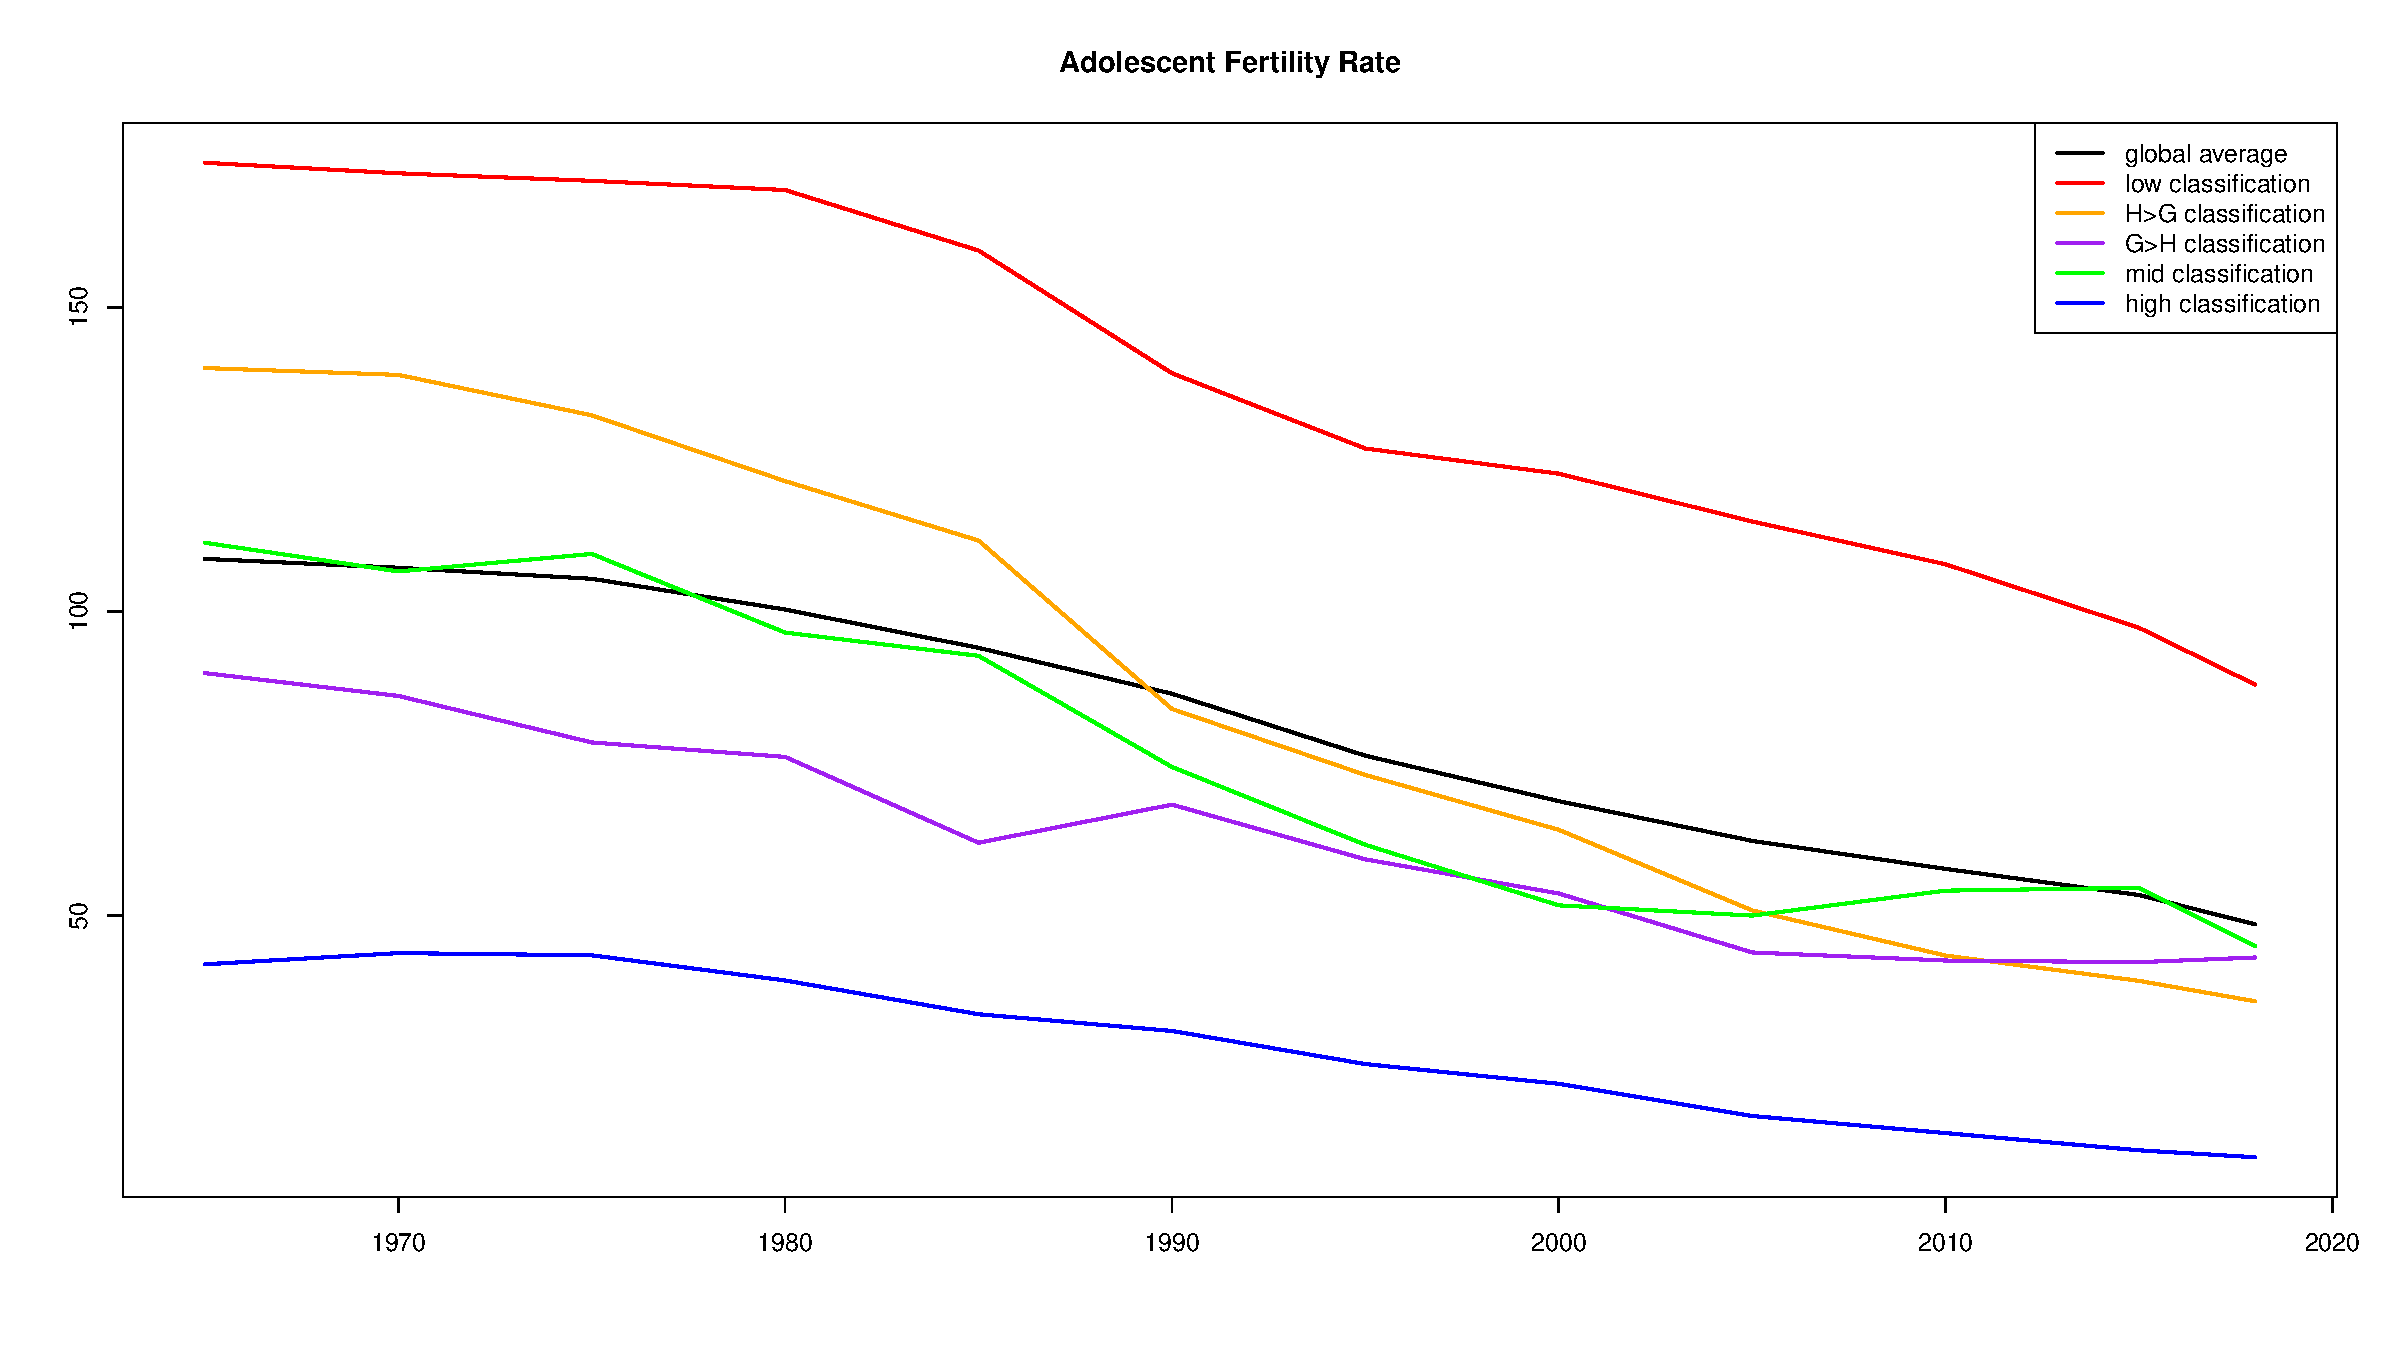
\includegraphics[width=\textwidth]{trend_asfr_adol_wpp.pdf}
\end{figure}

Plotting the averages of the health and gender variables at the global level and within the classification groups show clear improving trends over time (see Figures \ref{trends_life}-\ref{trends_afr}).\footnote{Note that here the original measures are shown as five-year averages, not the inverted versions used in the statistical analyses (see above). Also, the mean years of schooling ratio is available for a shorter time period, since 1990.}
First, there is considerable global improvement in the health and gender measures, regardless of how countries are classified.
Second, overall improvements are greatest in the low classifications, with some interesting differences. Most improvement in the IMR occurs in the \enquote{G>H} classification, and in the AFR occurs in the \enquote{H>G} classification, in both cases followed by the low classification group.
Improvements tend to be much less pronounced in the high classification.
This suggests possible ceiling effects for better performers that need to be accounted for in the analyses.
Other graphical analyses not shown here also indicate that low performers on the health and gender dimensions tend to have the most violence on average over time (across different measures and different types of violence), and high performers experience much less violence.\footnote{In a partial exception, average homicide rates are highest in intermediate rather than the lower classification groups, but the high classification clearly has the lowest average homicide rates.}

These classification groups are used in the analyses below to examine the possibility of vicious and virtuous cycles in two different ways, and these have different implications for how to conceptualize vicious and virtuous cycles. The simplest tests are whether the individual gender and health variables are positively correlated with each other or with violence variables (controlling for other factors), but in this approach, it is not possible to determine whether the gender, health and violence variables actually mutually reinforce each other in cycles. I use the classification groups for more direct tests.

First, to examine whether particular configurations of health and gender outcomes (i.e. classifications) are associated with improvements (or declines) in gender, health and violence variables, I include binary (\enquote{dummy}) variables indicating the groups based on \Cref{table_class}; this can be interpreted as an interaction effect of past health and gender outcomes on current health and gender outcomes or on violence outcomes. Here, associations of lower classifications with worse outcomes and of higher classifications with better outcomes would provide evidence that is consistent with \enquote{two-way} vicious or virtuous cycles, respectively.

Second, modelling interactions of these binary classification indicators with violence variables lets me calculate the statistical effects of past violence within classification groups on current health, gender or violence outcomes. This can be interpreted as a \enquote{three-way} cycle. We can test whether past violence in particular classification groups is associated with worse or better current health or gender outcomes or with more or less violence. For instance, if we find an association of past violence in lower classification groups with more current violence or worse health or gender outcomes, this evidence would support vicious cycles because violence begets more violence where countries perform comparatively poorly on health and gender. Or, if we find past violence in higher classifications groups is associated with better health or gender outcomes or less violence, this would support virtuous cycles, because countries in the classification groups were able improve conditions despite past violence. Moreover, the evidence does not need to be this clear-cut to be supportive of the vicious and virtuous cycles framework. For instance, past violence may be associated with more current violence across several or all classification groups, but more so in lower classification groups relative to higher ones; such evidence would also be supportive of vicious and/or virtuous cycles.

\section{Methods}
\label{methods}

In contrast to the cross-sectional models in the previous report (and reproduced in \Cref{appendix_cs_dane}), which examine the growth of the outcome variables between the periods 1991-1995 and 2011-2015, the panel models examine short-term changes from one five-year period to the next, over as many periods as data availability allows; they use so-called \enquote{wide} panels of many countries but only a small number of time periods (usually between 6 and 11 periods).
The dependent variables of the analyses are the individual health, gender, and violence variables.
I test the vicious and virtuous cycles hypotheses by examining the lagged gender or health variables, or the classification indicators, and the lagged violence variables or the interactions with the classification indicators, as explanatory variables.
All the panel models include covariates for logged GDP per capita, logged population size, and participatory democracy, in order to account for socio-economic and institutional conditions.\footnote{In the initial analyses, we also substituted other political regime variables, but only included participatory democracy in the final models because the others did not show statistical associations with the outcome variables. The new analyses continue this practice.}
I further include the lagged dependent variable in each model in order to account for trends, autocorrelation and ceiling effects.

When modelling the interactions, I also include additional models with controls for different types of violence.
I proxy the presence and magnitude of other types of violence with deaths rates for internal conflict (combatants and civilians), one-sided violence (civilians), and non-state conflict (combatants and civilians). For this purpose, I do not use the homicide rate for societal violence, because this has much more missing data points than the UCDP data.
To avoid introducing further endogeneity, I do not include deaths rates related to the violence variable of interest in a given model.
For instance, the models examining the role of internal conflict incidence do not include the closely related internal conflict death rate. Moreover, the models examining the role of repression or extra-judicial killings do not include the one-sided violence death rate because these measure overlapping phenomena. And models examining the role of homicides do not include the one-sided violence and non-state conflict death rates because these measures plausibly include at least some of the same deaths.

Analysis of observational data always requires careful attention to omitted variable biases and endogeneity of various kinds.
These issues become even more pressing concerns in panel data than in cross-sectional data, because of the lack of independence of observations within countries over time, leading to issues of correlated unit (country) effects, heteroscedasticity and serial correlation.
These are problems in our models and data, as evidenced by a variety of econometric tests developed for panel data, which we carried out for each regression equation to decide which estimators are most defensible.
This is important as the choice of estimator sometimes leads to different and even contradictory results.
Based on the results of these tests across models, we consider the fixed effects (FE, or "within") ordinary least squares estimator (OLS run on demeaned within-country data), and more preferably, the fixed effects general (or unrestricted) feasible generalized least squares (FEGLS) estimator.
Generally, the tests suggest that almost all models are subject to unit and/or time effects, and according to Hausman-test, random effects models are almost never justified. In many models, the tests further suggest persistent serial correlation, often of AR(1) type, leading to the preference for the FEGLS over the FE estimator, but the discussion below and the summary tables report both.

\section{* Analyses of health and gender outcomes *}
\label{results_hg}

This section and the next summarize the findings of the statistical analyses with illustrative examples. Details of all regression models and figures of all interaction effects are shown on the project website.\footnote{\href{https://timothoms.github.io/LSC-MWG/panel.html}{timothoms.github.io/LSC-MWG/panel.html}} Moreover, \Cref{appendix_tables} provides summary tables of the  findings of the main analyses across all outcome variables (but not for the analyses using longer lags or shortening the time period of the sample).
I report only associations that are statistically significant at the 0.05 alpha level or lower. As the regression figures on the project website, the figures of interactions effects below show effects with 95\% confidence intervals.
The discussion is organized by key independent variables to summarize their statistical associations across outcome variables, and focuses on the main models which include the classifications, explained in \Cref{data} and the control variables for types of violence. I only note the results for alternative timelines and lags where they diverge from the main findings.

\subsection*{Gender and health variables}

\todo[inline]{outcomes: Life Expectancy; IMR; UFMR; DALYs; MYS ratio; AFR; Labour participation ratio; GII; for each combination go through main findings and then alternative timelines if relevant; generally discuss overall findings with illustrative examples and refer to detailed findings in appendix and on website}

\subsection*{Classifications}
\subsection*{Internal Conflict}
\subsection*{State repression}
\subsection*{Non-state conflict}
\subsection*{Homicides}

\section{* Analyses of violence outcomes *}
\label{results_violence}

\todo[inline]{discuss classifications and violence controls; again, explain the logic of the research designs for violence outcomes: interactions are slightly different; organize by violence outcome; go through main findings and then alternative timelines (not applicable to robustness checks)}

\subsection*{Internal Conflict}
\subsection*{State repression}
\subsection*{Non-state conflict}
\subsection*{Homicides}

\section{* Discussion *}
\label{discussion}

\todo[inline]{discussion of new analyses and questions to address in the final report}

\section{* Sequencing analysis: work-in-progress *}
\label{sequencing}

As noted in \Cref{intro}, the Lancet Commission is interested in whether vicious and virtuous cycles are at work, but also if and how policy interventions to support gender equality and health equity can nudge societies into virtuous cycles. Toward this end, it would be useful to identify pathways of gender and health change to identify entry points and policy levers. A key question is: are there particular sequences of improvements in gender and health outcomes that are more likely to break countries out of vicious cycles? Therefore, another research stream is to map different pathways of change over time, subject to data availability, to determine which pathways are more common or likely to lead to improvements.

Initially, I mapped the trajectories based on the classifications explained in \Cref{data}, but have concluded that this is not a good representation of change over time, because for any given five-year period the classifications are relative to all other countries.\footnote{In the panel regression analyses, this is useful because it account for the global  improvements across the gender and health measures.} This means that an underlying change from one period to the next may not be reflected in the classifications, or a classification may change without a significant change in the underlying health and gender measures.

Therefore, I have also mapped the trajectories based on two of the underlying measures: the infant mortality rate (IMR) and the adolescent fertility rate (AFR). I consider these two variables, because the IMR is strongly correlated with life expectancy -- and thus they reveal similar information about trajectories -- and the other gender variable -- the mean years of schooling ratio of female to male -- is only available for a shorter period of time, whereas the AFR is available for the same countries and years as the IMR. This is a promising approach.
Figures of the trajectories for all countries in the dataset are shown on the project website.\footnote{\href{https://timothoms.github.io/LSC-MWG/sequencing.html}{timothoms.github.io/LSC-MWG/sequencing.html}. Note that starting points are indicated in red, while endpoints are shown in green. As in the statistical analyses, the IMR and AFR are inverted such that higher values indicate \enquote{better} outcomes.}
The next step is to determine whether a useful sequencing typology can be developed from this representation.

\clearpage
\appendix
\part*{Appendix}
\label{appendix}

\section{Summary tables for analyses extensions}
\label{appendix_tables}

Rather than presenting the many detailed regression tables here -- these details are available on the project website -- this appendix shows summary tables of statistically significant findings (at the 0.05 alpha level) of the main analyses. These show the outcome variables (DVs) in columns and key independent variables (IVs) in the rows, based on all models, with the following symbols indicating their statistical effects and specific notes; each cell in the table represents one or more separate models.

\begin{table}[!htb]
\centering
\caption{Legend}
\label{table_legend}
\begin{tabular}{ll}
\toprule
Symbol & Note \\
\midrule
$+$    & statistically significant positive effect \\
$-$    & statistically significant negative effect \\
$()$   & statistical effect not found in the preferred model (FEGGLS) \\
na     & variable not included in the model \\
DV     & variable is the DV \\
ref    & variable is the reference category \\
$[l]$  & effect is relative to the low classification \\
$[u]$  & effect is relative to the upper classification \\
$[v]$  & effect is present when accounting for other types of violence\\
\bottomrule
\end{tabular}
\end{table}

\begin{table}[!htbp]
\small
\centering
\caption{Health \& Gender Outcomes: base models}
\label{table_hg_base}
\begin{tabular}{lcccccccc}
\toprule
                          & Life              & IMR   & UFMR     & DALYs    & MYS    & AFR    & Labour        & GII \\
                          & Expectancy        &       &          &          &        &        & Participation & \\
                          &                   &       &          &          &        &        & Ratio         & \\
\midrule
lagged DV                 & $+$               & $+$   & $+$      & $+$      & $+$    & $+$    & $+$           & $+$ \\
Life Expectancy           & DV                & na    & na       & na       &        & $+$    &               & \\
Infant Mortality          & na                & DV    & na       & na       &        & $+$    &               & $+$ \\
MYS Ratio                 & $+$               & $+$   & $(+)$    & $+$      & DV     & na     & na            & na \\
Adolescent Fertility Rate & $+$               & $-$   & $-$      & $-$      & na     & DV     & na            & na \\
low classification        & $-$[u]            &       &          &          & $-$[u] & $-$    &               & \\
H>G classification        & $(+)$[l]          &       &          & $(-)$[l] & $+$[l] & $-$[u] &               & \\
G>H classification        & $(-)$[u] / $+$[l] & $(-)$ & $(-)$[u] &          &        & $+$[l] & $-$[l]        & \\
mid classification        & $+$[l]            &       &          & $(-)$[l] & $+$[l] & $+$[l] &               & \\
upp classification        & $+$[l]            &       &          &          & $+$[l] & $+$[l] &               & \\
\bottomrule
\end{tabular}
\end{table}

\begin{landscape}
\begin{table}[!htbp]
\centering
\caption{Health \& Gender Outcomes: Findings on Internal conflict}
\label{table_hg_conflict}
\begin{tabular}{lcccccccc}
\toprule
                         & Life       & IMR      & UFMR     & DALYs    & MYS    & AFR               & Labour        & GII \\
                         & Expectancy &          &          &          &        &                   & Participation & \\
                         &            &          &          &          &        &                   & Ratio         & \\
\midrule
Conflict                 & $+$        &          &          & $+$      &        &                   & $-$[v]        & $+$ \\
--- low interaction      & $+$        &          &          &          &        &                   &               & $(+)$[v] \\
--- H>G interaction      & $(+)$      & $+$      &          &          &        & $-$               &               & $+$[v] \\
--- G>H interaction      &            & $-$      &          & $(+)$[v] &        &                   & $(-)$[v]      & \\
--- mid interaction      &            &          & $(+)$    &          &        & $(-)$[v] / $+$[v] &               & $+$[v] \\
--- upp interaction      &            &          &          &          &        &                   & $-$[v]        & \\
Conflict Deaths          &            & $-$      & $-$      & $+$      &        & $+$               &               & \\
--- low interaction      & $-$[v]     & $-$      & $(-)$    & $+$      &        & $(-)$[v] / $+$[v] &               & \\
--- H>G interaction      &            &          &          &          &        & $+$[v]            &               & \\
--- G>H interaction      & $-$[v]     & $-$[v]   & $(-)$[v] &          &        & $(+)$[v] / $-$[v] &               & $-$[v] \\
--- mid interaction      &            &          &          & $(+)$[v] & $-$[v] & $-$[v]            &               & $(+)$[v] \\
--- upp interaction      &            &          &          & $+$      &        & $(-)$[v]          &               & \\
Conflict Civilian Deaths & $+$        &          &          & $+$      &        & $+$               &               & \\
--- low interaction      & $+$        &          &          & $+$[v]   &        & $+$               &               & $-$[v] \\
--- H>G interaction      &            &          &          &          &        &                   &               & \\
--- G>H interaction      & $-$[v]     & $-$[v]   & $-$[v]   &          &        & $-$[v]            &               & \\
--- mid interaction      &            & $(-)$[v] &          & $(+)$[v] &        & $-$[v]            &               & \\
--- upp interaction      &            & $+$[v]   &          & $+$      &        &                   &               & \\
\bottomrule
\end{tabular}
\end{table}
\end{landscape}

\begin{landscape}
\begin{table}[!htbp]
\centering
\caption{Health \& Gender Outcomes: Findings on State Repression}
\label{table_hg_repression}
\begin{tabular}{lcccccccc}
\toprule
                    & Life           & IMR                     & UFMR           & DALYs    & MYS    & AFR                     & Labour        & GII \\
                    & Expectancy     &                         &                &          &        &                         & Participation & \\
                    &                &                         &                &          &        &                         & Ratio         & \\
\midrule
OSV                 &                & $(-)$                   & $(-)$          &          &        &                         &               & \\
--- low interaction &                & $-$[v]                  & $-$ / $(-)$[v] &          & $+$[v] & $+$[v]                  &               & \\
--- H>G interaction &                &                         &                &          &        &                         &               & $+$[v] \\
--- G>H interaction & $+$[v]         &                         &                &          &        &                         &               & \\
--- mid interaction & $+$ / $(+)$[v] &                         &                &          & $-$[v] & $(-)$[v]                &               & \\
--- upp interaction &                &                         &                & $(+)$    &        &                         &               & \\
OSV Deaths          & $+$            & $(-)$                   & $(-)$          & $+$      &        & $+$                     &               & \\
--- low interaction & $+$[v]         & $(-)$(low)              & $(-)$          & $+$[v]   &        & $+$                     & $(+)$         & \\
--- H>G interaction &                &                         &                &          &        &                         &               & \\
--- G>H interaction &                & $(-)$                   & $(-)$          &          & $+$[v] &                         &               & $-$[v] \\
--- mid interaction & $+$[v]         &                         &                &          & $-$[v] & $(-)$[v]                &               & \\
--- upp interaction & $(+)$[v]       &                         &                & $(+)$[v] &        &                         & $-$           & \\
LPI                 &                & $+$                     & $+$            & $+$      &        & $(+)$                   & $(-)$         & $+$ \\
--- low interaction &                & $-$[v]                  & $-$[v]         &          &        & $+$ / $(-)$[v] / $-$[v] &               & \\
--- H>G interaction &                & $+$ / $(+)$[v] / $-$[v] & $+$ / $(+)$[v] & $(+)$[v] & $-$[v] & $(+)$ / $-$[v]          &               & $+$[v] \\
--- G>H interaction & $+$[v]         & $+$[v]                  & $+$            & $+$      & $-$[v] & $+$[v]                  &               & \\
--- mid interaction &                & $+$ / $(+)$[v]          & $+$ / $(+)$[v] & $(+)$[v] & $-$[v] &                         &               & \\
--- upp interaction & $(-)$ / $-$[v] & $+$ / $(+)$[v]          & $+$ / $(+)$[v] & $(+)$[v] &        & $(+)$[v] / $-$[v]       & $(-)$[v]      & $+$[v] \\
Killings            &                &                         &                &          &        &                         &               & \\
--- low interaction &                & $(-)$ / $-$[v]          & $(-)$          & $-$[v]   &        & $-$[v]                  &               & \\
--- H>G interaction &                & $+$                     & $+$ / $(+)$[v] & $(+)$[v] &        & $-$[v]                  &               & \\
--- G>H interaction & $(+)$          &                         &                & $(+)$[v] &        &                         &               & \\
--- mid interaction &                & $+$ / $(+)$[v]          & $+$            & $(+)$[v] &        &                         &               & $(+)$[v] \\
--- upp interaction &                & $(+)$[v]                & $(+)$          &          &        & $(+)$                   &               & \\
\bottomrule
\end{tabular}
\end{table}
\end{landscape}

\begin{landscape}
\begin{table}[!htbp]
\centering
\caption{Health \& Gender Outcomes: Findings on Societal Violence}
\label{table_hg_societal}
\begin{tabular}{lcccccccc}
\toprule
                    & Life       & IMR            & UFMR           & DALYs             & MYS      & AFR            & Labour        & GII \\
                    & Expectancy &                &                &                   &          &                & Participation & \\
                    &            &                &                &                   &          &                & Ratio         & \\
\midrule
NSC                 &            &                &                & $+$               &          & $+$            &               & \\
--- low interaction &            &                &                & $+$               &          & $+$[v]         &               & $-$[v] \\
--- H>G interaction &            & $(-)$          & $(-)$          &                   &          & $+$[v]         &               & $-$ \\
--- G>H interaction &            &                &                &                   &          &                &               & \\
--- mid interaction &            &                &                &                   &          &                & $(-)$[v]      & \\
--- upp interaction &            &                &                &                   & $(+)$[v] & $+$[v]         &               & \\
NSC Deaths          & $+$        &                &                & $+$               &          & $+$            &               & \\
--- low interaction & $+$        & $+$[v]         & $+$[v]         & $+$               & $+$[v]   & $+$[v]         &               & \\
--- H>G interaction &            & $(-)$[v]       & $(-)$[v]       &                   &          & $+$[v]         &               & \\
--- G>H interaction & $(-)$      & $(-)$[v]       &                &                   &          & $(+)$[v]       &               & $-$[v] \\
--- mid interaction & $(+)$[v]   &                &                &                   &          &                & $(-)$         & \\
--- upp interaction &            & $(+)$[v]       & $(+)$[v]       & $(+)$[v]          &          & $(+)$[v]       &               & \\
NSC Civilian Deaths & $+$        &                &                & $+$               &          & $+$            & $(+)$         & \\
--- low interaction & $+$        & $+$[v]         &                & $+$               &          & $+$[v]         & $(+)$[v]      & \\
--- H>G interaction &            & $(-)$ / $-$[v] & $(-)$[v]       & $(-)$[v]          &          &                & $(-)$[v]      & \\
--- G>H interaction & $+$[v]     & $+$            & $+$[v]         & $(-)$[v] / $+$[v] &          &                & $(+)$[v]      & \\
--- mid interaction &            &                &                &                   &          &                &               & \\
--- upp interaction & $(+)$[v]   & $(+)$[v]       & $(+)$[v]       & $(+)$[v]          & $(-)$    & $+$[v]         & $(+)$[v]      & $(+)$ \\
Homicides           & $-$        & $+$            & $+$            & $(-)$             &          & $+$            &               & \\
--- low interaction & $-$[v]     & $-$[v]         & $+$ / $-$[v]   & $-$[v]            &          & $-$[v]         & $+$[v]        & $-$[v] \\
--- H>G interaction & $(-)$[v]   &                & $+$            &                   &          & $-$[v]         &               & \\
--- G>H interaction & $-$[v]     & $+$            &                & $-$[v]            &          & $-$[v]         & $+$[v]        & $-$[v] \\
--- mid interaction & $(-)$[v]   & $-$[v]         & $(-)$[v] / $+$ & $(-)$[v]          &          &                & $+$[v]        & \\
--- upp interaction & $(-)$[v]   & $+$[v]         & $+$[v]         &                   &          & $+$ / $(+)$[v] & $-$[v]        & $+$[v] \\
\bottomrule
\end{tabular}
\end{table}
\end{landscape}

\begin{landscape}
\begin{table}[!htbp]
\centering
\caption{Violence Outcomes}
\label{table_violence}
\begin{tabular}{lccccccccccc}
\toprule
                          & Conflict       & Conflict & Civilian & OSV    & OSV    & LPI    & Killings & NSC      & NSC      & NSC      & Homicides \\
                          &                & Deaths   & Deaths   &        & Deaths &        &          &          & Deaths   & Civilian & \\
                          &                &          &          &        &        &        &          &          &          & Deaths   & \\
\midrule
Life Expectancy           &                &          & $+$      & $-$    &        & $+$    &          &          &          &          & \\
Infant Mortality          & $-$            &          &          & $(-)$  &        & $(-)$  &          &          &          &          & \\
MYS Ratio                 &                &          &          &        & $-$    & $-$    &          &          &          &          & \\
Adolescent Fertility Rate & $-$            &          &          &        &        & $+$    & $(+)$    &          &          &          & $+$ \\
low classification        & ref            & ref      & ref      & ref    & ref    & ref    & ref      & ref      & ref      & ref      & ref \\
H>G classification        &                & $-$      &          &        &        & $+$    &          & $+$      & $-$      &          & \\
G>H classification        &                &          &          &        &        & $+$    &          & $+$      & $-$      &          & \\
mid classification        &                & $-$      &          &        &        & $+$    &          & $+$      & $-$      &          & \\
upp classification        &                & $-$      & $-$      &        &        & $+$    &          & $+$      & $-$      &          & \\
lagged DV                 & $+$            & $+$      & $+$      & $+$    &        & $+$    & $+$      & $(+)$    & $+$      & $+$      & $+$ \\
--- low interaction       & $+$[v]         & $+$[v]   & $+$[v]   & $+$[v] &        & $+$[v] & $+$[v]~  &          & $+$[v]   & $+$[v]   & $+$ / $-$[v]~ \\
--- H>G interaction       & $+$            & $+$[v]   & $(-)$[v] & $(+)$  &        & $+$[v] & $+$[v]~  & $+$[v]   & $(+)$[v] &          & $+$[v]~ \\
--- G>H interaction       & $+$ / $(+)$[v] & $(+)$[v] &          &        &        & $+$[v] & $+$[v]~  &          &          &          & $+$~ \\
--- mid interaction       & $+$            & $-$[v]   &          & $+$[v] &        & $+$[v] & $+$[v]   &          & $(+)$[v] &          & $+$[v]~ \\
--- upp interaction       & $+$ / $(+)$[v] &          &          & $+$    &        & $+$[v] & $+$[v]   & $(+)$[v] &          &          & $+$ / $-$[v]~ \\
\bottomrule
\end{tabular}
\end{table}
\end{landscape}


\section{Cross-sectional analyses in the previous report}
\label{appendix_cs_dane}

This section reproduces the discussion of the cross-sectional analyses in the previous report, authored by Dane Rowlands.

\subsection{Methods}

The cross-sectional regression analyses examine longer-term effects.
% of key health and gender variables and a measure of cumulative violence or conflict on the improvements in country performance from 1996 to 2015 in each of the health and gender outcomes.
The dependent variables are the improvements (increase from the 1996 start period to the 2015 end period) in country performance from 1996 to 2015 for each measure of health and gender performance, and a measure of cumulative violence or conflict over the same time-period.
The key explanatory variables are the values of the different dependent variables representing conditions prior to, or in, 1995, as well as the control variables for the level and subsequent changes in per capita income and political structure, and for the subsequent presence of conflict. The time structure of the analysis means that the regressions are essentially testing for any consistent and significant statistical relationships indicating a possible direct association between future health, gender, and conflict performance over a long (twenty year) period, starting conditions of health, gender, conflict, economic and political conditions, and indirect connections through subsequent economic, political, and conflict developments. Using the cross-section analysis and the long time period means that we are examining longer-term trends rather than year-to-year variation. The structure also minimizes the likelihood of reverse causality and endogeneity, and versions of the regressions are essentially trying to predict future performance using only prior information.

These key regression equations are also supplemented by similar equations to examine the factors associated with economic improvements over the 1996-2015 period, and changes in political structure. This analysis tests for potential indirect associations between different performance measures. For example, a direct association would be suggested by the analysis if initial gender or health performance is related to subsequent improvements in those measures. An indirect relationship might be suggested if, instead, subsequent improvements in gender or health over the long term are only related to economic, political, or conflict patterns over the long run as well, but that these are in turn influenced by initial health and gender performance. So the causal route from better initial gender performance to improved health performance might not be directly from gender to health, but through initial gender conditions affecting subsequent economic performance, which in turn affects health performance.

% As part of the analyses, standard diagnostics on heteroscedasticity and multicollinearity are examined and the sensitivity of the results are assessed with variations in the regression equations, sample size and variable forms in a step-wise process.
Finally, the process of narrowing down the most informative regressions is extensive. In addition to standard diagnostics on heteroscedasticity and multicollinearity, several versions of the regressions are examined to gauge the sensitivity of the results to variations in the equation, included observations, and variable forms. Due to the presence of multicollinearity in some cases, and since the number of observations is occasionally fairly small, variables with statistically insignificant coefficient estimates are removed from the equations to test for the sensitivity of results. This step-wise process is carefully scrutinized at each step to avoid cherry-picking results and to ensure that the reported results are robust to most changes. We also drop some variables for theoretical reasons, and this process is often quite informative in identifying potentially important associations. We clearly identify the inferences associated with these changes.

\subsection{Health and Gender Outcomes}

There are two important observations on the data that need to be recognized. First, on average most of the key indicators of health and gender exhibit steady improvement over the 1995-2015 period both in aggregate and for almost all countries in the sample. As a result, in the cross-section analysis virtuous circles and vicious circles are essentially opposite sides of the same coin as the performance of countries are essentially measured relative to one another. The \enquote{virtuous} group performing relatively well in terms of future performance (virtuous circle) implies that the \enquote{vicious} group is performing relatively poorly (vicious circle). One line of inquiry that might be worth pursuing is to impose an absolute measure, for example sustained declining performance, and ask which country groups exhibit absolute decline. In the cross section data it is rare that well-off countries end up having sustained reduction in health and gender performance, while poorly-off countries exhibit a much broader range of future performance, ranging from sustained declines to dramatic improvements.

In addition, the pace of improvement tends to be significantly faster for those countries that have poorer initial performance in these categories. This pattern suggests the presence of a \enquote{ceiling effect}: those countries that have already achieved high performance in health and gender equality have very little room for additional improvement, while those with weak initial performance have ample scope for improvement. The presence of a ceiling effect complicates the analysis considerably, since the data will tend to suggest the opposite of virtuous and vicious circles simply because initially poor performers will find it far easier to outperform initially strong ones. An alternative interpretation of this robust result is the convergence hypothesis whereby poorer performers generally tend to catch up with the top performers. Differentiating between the two interpretations is difficult, since both are plausible. We conduct a preliminary investigation of this problem by doing supplementary analysis using improvement measures that are adjusted for initial conditions. In effect, this supplementary analysis asks how countries with better gender or health measures perform relative to comparable countries in terms of income per capita.

The use of per capita income to adjusted performance expectations is linked to the second key observation: countries with higher per capita income also tend to have better initial measures of for health, gender, conflict and violence, and democracy. These strong cross-variable correlations mean that there is often considerable multicollinearity in the model, especially between health and gender variables, as well as with lower levels of violence. This static correlation is indeed suggestive of virtuous and vicious circles, but it does not imply a direct causal and dynamic relationship. Instead, it may simply be the case that a single common variable, such as economic performance, causally affects these measures in the same way. The regression analysis is structured to address this problem, though imperfectly.

\Cref{table_cs_hg} presents the coefficient estimates from the regressions examining improvements in the health and gender outcomes. The first two columns show the results for changes in life expectancy; the reported results are representative of the analysis of life expectancy, and illustrative of many of the findings of other performance measures as well.\footnote{Recall that some variables have been rescaled so that an increase in any health or gender measure represents an improvement in performance; for example, infant mortality has been inverted so that when the measure of infant mortality increases, it represents a decline in infant mortality rates. The only variables where an increase is \enquote{bad} are the conflict and violence measures.}

\begin{landscape}
\begin{table}[!htbp]
\footnotesize
\centering
\caption{Health and Gender Equality Improvements (change during 1995-2015)}
\label{table_cs_hg}
\begin{tabular}{lcccccccc}
\toprule
                               & Life Expectancy & Life Expectancy & IMR         & IMR        & MYS Ratio       & MYS Ratio   & AFR        & AFR\\
                               & base            & prediction      & base        & prediction & base            & prediction  & base       & prediction \\
\midrule
Life expectancy 1995           & -0.302 †        & -0.259 †        &             &            &                 &             &            & \\
                               & (0.074)         & (0.080)         &             &            &                 &             &            & \\
Infant mortality rate 1995     & -0.0643 **      & -0.0606 **      & -0.628 ***  & -0.583 *** &                 &             & 0.136 **   & 0.151 **\\
                               & (0.012)         & (0.016)         & (0.000)     & (0.000)    &                 &             & (0.017)    & (0.013) \\
Adolescent fertility rate 1995 & 0.0506 **       & 0.0449 **       & 0.123 ***   & 0.0962 *   & 0.000588 **     & 0.00062 *   & -0.265 *** & -0.271 ***\\
                               & (0.013)         & (0.011)         & (0.009)     & (0.032)    & (0.023)         & (0.017)     & (0.000)    & (0.000) \\
Gender schooling ratio 1995    &                 &                 &             &            & -0.368 ***      & -0.354 ***  &            & \\
                               &                 &                 &             &            & (0.000)         & (0.000)     &            & \\
Conflict measure 1989-1995     & 0.0601 †        & 0.0318 †        &             &            & 0.000532 †      & -0.000365 † &            & \\
                               & (0.091)$^a$     & (0.093)$^c$     &             &            & (0.083)$^c$     & (0.079)$^c$ &            & \\
Conflict measure 1996-2015     & -0.193 *        &                 &             &            & -0.012 ***      &             &            & \\
                               & (-0.049)$^{b,r}$&                 &             &            & (0.003)$^{c,r}$ &             &            & \\
GDPpc 1995                     &                 &                 & -0.2361 *** &            &                 &             &            & \\
                               &                 &                 & (0.009)     &            &                 &             &            & \\
GDPpc growth 1996-2015         & 0.0630 ***      &                 & 0.137 *     &            &                 &             &            & \\
                               & (0.008)         &                 & (0.027)     &            &                 &             &            & \\
Past Polyarchy 1991-1995       &                 & 4.22 ***        & 8.97 **     &            &                 & -0.0558 †   &            & -16.92 † \\
                               &                 & (0.003)         & (0.02)      &            &                 & (0.071)     &            & (0.052) \\
Future Polyarchy 1996-2015     & 4.80 ***        &                 &             &            & -0.0619 *       &             & -16.37 **  & \\
                               & (0.002)         &                 &             &            & (0.041)         &             & (0.024)    & \\
Constant                       & 22.8 †          & 21.1 †          & -1.30       & 1.824 *    & 0.470 ***       & 0.452 ***   & 16.4 ***   & 16.13 *** \\
                               & (0.072)         & (0.060)         & (0.676)     & (0.05)     & (0.000)         & (0.000)     & (0.000)    & (0.002) \\
\midrule
Sample size                    & 156             & 165             & 156         & 180        & 135             & 135         & 165        & 165 \\
$R^2$                          & 0.492           & 0.483           & 0.824       & 0.817      & 0.521           & 0.510       & 0.344      & 0.344 \\
F-test $p$-value               & 0.000           & 0.000           & 0.000       & 0.000      & 0.000           & 0.000       & 0.000      & 0.000 \\
\bottomrule
\end{tabular}
\caption*{P-values in parentheses, derived from robust standard errors; ***, **, *, † indicate statistical significance at the 0.01, 0.025, 0.05 and .10 levels respectively; $^a$ internal conflict indicator; $^b$ civilian death rate from internal conflict; $^c$ civilian death rate from one-sided-violence; $^r$ robust to variations in the other conflict measure.}
\end{table}
\end{landscape}


The base model (column 1) provides the results for the best, most representative stepwise reduced estimating equation. The negative coefficient on both the life expectancy and infant mortality variables is indicative of the common \enquote{ceiling effect} observed in almost all of the regressions. Essentially, if a country is already performing well in terms of health performance, that country is likely to have little room for significantly better performance. For each one-year increase in life expectancy in 1995, the increase in life expectancy over the next 20 years declines is 0.3 years lower; the effect of a decline of one infant death per 1000 is to lower future life expectancy improvement by 0.064 years over the next 20 years.

A result that appeared quite robustly in the different regressions was the positive association between improvements (numerical declines) in the adolescent fertility rate of a country, and subsequent improvements in life expectancy. This association indicates that if the number of children born per 1000 adolescent girls fell by one, future life expectancy would improve by .05 years. The association could be indicative of a broad virtuous relationship between better overall rights for women (to the extent that these are primary factors in decreasing teenage pregnancy), or it could be more directly causal in the sense that reduced physical and emotional stress from adolescent pregnancy and childbirth may increase future life expectancy for a girl as she ages. The robust association, however, is encouraging.

The conflict and violence variables have the expected relationship with life expectancy improvements but are complex. A sensible and fairly robust pattern emerged from the regression analysis: previously high rates of conflict or violence tended to be associated with future improvement in life expectancy, which is possible if previous conflict had artificially reduced life expectancy levels below what would otherwise have been the case. Subsequent life expectancy improvements, therefore, might simply reflect the reversion to expected levels after a conflict ends. By contrast, measures of conflict or violence over the period for which life expectancy improvements are being measured are associated with declines in that improvement, which is again sensible. In some regressions, removing the future conflict and violence measure often led to a reversal of signs for the previous conflict and violence measure, which we think is due to the tendency for violence to have a high degree of inertia, so that the decline in life expectancy is reflecting the likely presence of future conflict, not the presence of past violence.

The economic and political control variables all have plausibly signed, coefficient estimates. Future economic growth and future high levels of democratic performance are both associated with improvements in life expectancy over the same period. Finally, the equation as a whole performs remarkably well, explaining almost half of the cross-sectional variance in life expectancy improvement for a sample of 156 countries.

When the life expectancy measure in 1995 is removed from the estimating model (not shown)
% (Table 1, Model 2)
to ensure no spurious connection between the dependent variable and its lag, the ceiling effect is still present as indicated in the negative association with the remaining health measure (infant mortality), since these health measures are highly correlated (0.96). The other results are fairly comparable except that the polyarchy measure that retains its statistical significance switches from the future values to the prior value. While this equation instability suggests that some caution is warranted in making inferences about the relationship between political structure and life expectancy, it is the case that there is a high degree of continuity in the polyarchy measure, with the pre- and post-1995 measures having a correlation of 0.9. Finally, there is only a small loss in explanatory power as represented by the $R^2$ value.

The model variant in the second column uses only pre-1996 variables to generate a prediction of post-1995 life expectancy improvement. The results are comparable to those of the previous, and while the sample increases slightly, the proportion of variance explained in the model remains very high (0.48). Finally, another model (not shown) examined the improvement in life expectancy adjusted for a country's initial life expectancy level and initial per capita income. While this form of the dependent variable yields a very different measure (the correlation between the actual improvement and the adjusted measure is only 0.08), the results are remarkably similar in terms of the explanatory variables with statistically significant coefficient estimates, and the sign and magnitude of those estimates. The main difference is that lower prior per capita income is associated with better subsequent improvement, which is consistent with a recovery in life expectancy from previously lower than expected levels.

Overall, the analysis of life expectancy improvement suggests the following important relationships. First, there appears to be a strong ceiling effect in which previously good performance on health measures limits the scope for future improvement. Second, lower levels of adolescent fertility rates (AFR) in the past are consistently linked with better future life expectancy improvements. While AFR may reflect both health and gender balance conditions, the relationship is consistent with the virtuous circle concept, and possibly the importance of gender balance as a factor in future health improvements. Past conflict is associated with subsequent life expectancy improvement, which is presumably because of its effect on suppressing the starting point for measuring future improvement. Future conflict, however, clearly suppresses future life expectancy. There is also evidence that democracy is associated with improved life expectancy performance, as is economic growth.

The analysis for infant mortality rate is generally consistent with the findings for life expectancy. The third and fourth columns in \Cref{table_cs_hg} present the key results. As with life expectancy, in both the base model and the predicting model there is a strong ceiling effect, but also a strong positive connection to previously lower rates of adolescent fertility. There is no strong and consistent link to prior or future conflict. Democracy is positively associated with improvements in infant mortality. There is weak evidence that poor prior economic performance, and better future economic performance, are linked to infant mortality rate improvements. These two variables are themselves correlated (0.56) though the evidence of strong multicollinearity in the equation is weak, and when one is removed from the equation the statistical significance of the coefficient estimate for the other drops below acceptable levels, while the other coefficient estimates remain qualitatively unchanged. So, there is a need to treat the relationship between income per capita measures and infant mortality improvements with some caution. Both the base equation and the predictive equation have very high rates of explanatory power, with the $R^2$ being about 0.82 in both cases.

The estimations for improvements in gender schooling years ratios and adolescent fertility rates are presented in the remaining columns. The results all point to the presence of a ceiling effect (i.e. a consistent negative relationship between the previous level and the future improvement rate). There is no evidence that either of the health measures affects the schooling measure, but solid evidence of a positive link between infant mortality rates and future AFR improvements. Conflict affects schooling improvements in the same way as life expectancy: past conflict is associate with future improvements (attributed to catch up) and future violence is associated with lower improvements in female-to-male ratios of schooling years. The one anomaly is in the prediction model for gender balance in schooling, where current conflict is negatively associated with improvements. The likely reason for this reversal is the strong inertia in conflict measures, with past violence being highly correlated with future conflict (correlation = 0.69), so when future conflict is not included in the equation its effect is transferred to the associated past measure. Neither gender-related variable is associated with economic performance. The only unexpected effect is the frequent, though often statistically marginal, negative relationship between democracy and future improvements in both gender measures. This result requires future investigation.

\subsection{Violence Outcomes}

The analysis so far has focused on the possible direct effects of prior gender and health performance on their future improvements, controlling for key characteristics of conflict, the economy, and political structure. These last three variables may also provide indirect channels for affecting the future. Health and gender levels could amplify their effects through these key controls. To investigate these potential indirect connections we use regression analysis to estimate the association between past health and gender measures and future conflict, economic growth, and political structure.

\begin{table}[!htb]
\centering
\caption{Predicting future conflict/violence phenomena (1996-2015)}
\label{table_cs_violence}
\begin{tabular}{lccccc}
\toprule
                               & Future          & Future          & Future      & Future     & Future \\
                               & Internal        & Internal        & Internal    & Civilian   & Civilian \\
                               & Conflict        & Conflict        & Conflict    & Deaths     & Deaths\\
                               & Years           & Years           & Years       & (Conflict) & (OSV) \\
\midrule
Life expectancy 1995           & -0.103 ***      &                 &             &            & \\
                               & (0.000)         &                 &             &            & \\
Infant mortality rate 1995     &                 & -0.0265 ***     &             &            & \\
                               &                 & (0.000)         &             &            & \\
Mean years schooling 1995      &                 &                 & -5.00 ***   & -2.20 *    & -1.422 *** \\
                               &                 &                 & (-0.010)    & (0.030)    & (0.010) \\
Lagged dependent variable      & 0.407 ***       & 0.404 ***       & 0.374 ***   &            & 0.0683 *** \\
                               & (0.000)         & (0.000)         & (0.000)     &            & (0.000) \\
Constant                       & 7.71 ***        & -0.248          & 5.27 ***    & 0.549 *    & 1.37 *** \\
                               & (0.000)         & (0.498)         & (0.003)     & (0.034)    & (0.008) \\
\midrule
Sample size                    & 180             & 180             & 143         & 143        & 143 \\
$R^2$                          & 0.471           & 0.473           & 0.413       & 0.013      & 0.54 \\
F-test $p$-value               & 0.000           & 0.000           & 0.000       & 0.030      & 0.000 \\
\bottomrule
\end{tabular}
\caption*{P-values in parentheses, derived from robust standard errors; ***, **, *, † indicate statistical significance at the 0.01, 0.025, 0.05 and .10 levels respectively.}
\end{table}


A key set of relationships for our work involves health, gender, and violent conflict. We investigated several measures of violence in our analysis, including in the previous regressions on health and gender improvements. Here, the primary violence indicators we use are a count measure for the number of years a country experiences violent conflict, a measure of the number of civilian deaths from internal conflict, and the number of civilian deaths associated with one-sided violence. All the future cumulative values of these three variables for the 1996-2015 period are positively correlated with each other and negatively correlated with the past measures of the heath and gender variables in the analysis. The formal regression analysis uses these future violence variables as the dependent variable, while the explanatory variables are past health and gender measures, the lagged dependent variable, and measures of economic performance and political structure. Some illustrative results are presented in \Cref{table_cs_violence}.

In the prediction of future violence the results were consistent. In all cases the best step-wise reduced equation includes one of the health and gender measures, often along with the lagged version of the dependent variable. Past education balance is significantly associated with all three future violent conflict measures, and all four health and gender measures are associated significantly with future death rates from one-sided violence. Both health measures are also statistically significantly associated with the variable measuring the number of conflict years, but not civilian deaths from internal conflict. Therefore, there is considerable evidence that better performance in health and gender generally is associated with fewer future deaths, which in turn is often associated with greater improvements in health and gender in the future.

The analyses of future economic growth and future levels of democracy suggest that these indirect channels have very little role to play (not shown). Current health and gender measures do not appear to be significantly associated with either the economy or political structure, with the exception of a weak relationship between life expectancy and future economic growth.

\section{Panel analyses in the previous report}
\label{appendix_panel}

\subsection{Health and gender outcomes}

Rather than presenting the many detailed regression tables of these analyses, we show summary tables of statistically significant findings (at the 0.05 alpha level). The summary tables in this section show the outcome variables (DVs) in columns and explanatory variables and covariates (IVs) in the rows, such that each cell represents a separate statistical model. Statistically positive and negative effects are indicated by \enquote{$+$} and \enquote{$-$}, respectively, and \enquote{$[]$} indicates associations that contradict our expectations. Effects found in FE OLS estimations but not in the preferred FE GGLS estimations are indicated by \enquote{$()$}; we consider this weaker evidence.
\Cref{table_panel_gh} shows the findings of the models with health or gender dependent variables.

\begin{table}[!htbp]
\footnotesize
\centering
\caption{Summary of Previous Findings on Health and Gender Outcomes}
\label{table_panel_gh}
\begin{tabular}{lc|c|c|c}
\toprule
                                           & Life       & IMR     & MYS     & AFR \\
                                           & Expectancy &         & Ratio   & \\
\midrule
Life Expectancy                                   & $+$   & na      &         & $+$ \\
Infant Mortality                                  & na    & $+$     &         & $+$ \\
Mean Years of Schooling ratio                     & $+$   & $+$     & $+$     & na \\
Adolescent Fertility Rate                         & $+$   & $[-]$   & na      & $+$ \\
low classification                                & $-$   & $-$     & $-$     & $-$ \\
high classification                               &       &         &         & \\
Conflict                                          & $[+]$ &         &         & \\
\qquad Conflict: low interaction                  &       &         &         & \\
\qquad Conflict: high interaction                 &       & $+$     &         & \\
War                                               &       &         &         & $-$ \\
\qquad War: low interaction                       &       &         &         & \\
\qquad War: high interaction                      &       &         &         & \\
Conflict Deaths                                   &       & $-$     &         & $[+]$ \\
\qquad Conflict Deaths: low interaction           &       &         &         & $[+]$ \\
\qquad Conflict Deaths: high interaction          &       &         &         & \\
Conflict Civilian Deaths                          & $[+]$ &         &         & $[+]$ \\
\qquad Conflict Civilian Deaths: low interaction  & $[+]$ &         &         & $[+]$ \\
\qquad Conflict Civilian Deaths: high interaction &       &         &         & \\
OSV                                               &       & $(-)$   &         & \\
\qquad OSV: low interaction                       &       & $(-)$   & $[+]$   & $[+]$ \\
\qquad OSV: high interaction                      &       &         &         & \\
OSV Deaths                                        & $[+]$ & $(-)$   &         & $[+]$ \\
\qquad OSV Deaths: low interaction                &       &         &         & \\
\qquad OSV Deaths: high interaction               &       &         &         & \\
NSC                                               &       &         &         & $[+]$ \\
\qquad NSC: low interaction                       &       &         &         & \\
\qquad NSC: high interaction                      &       &         &         & \\
NSC Deaths                                        & $[+]$ &         &         & $[+]$ \\
\qquad NSC Deaths: low interaction                &       &         &         & \\
\qquad NSC Deaths: high interaction               &       & $[(+)]$ &         & \\
NSC Civilian Deaths                               & $[+]$ &         &         & $[+]$ \\
\qquad NSC Civilian Deaths: low interaction       &       &         &         & \\
\qquad NSC Civilian Deaths: high interaction      &       &         & $[(-)]$ & \\
LPI                                               &       & $[+]$   & $-$     & $[(+)]$ \\
\qquad LPI: low interaction                       &       &         &         & \\
\qquad LPI: high interaction                      &       & $(+)$   &         & \\
Torture                                           &       &         &         & \\
\qquad Torture: low interaction                   &       &         &         &   \\
\qquad Torture: high interaction                  &       & $(+)$   &         & \\
Killings                                          &       &         &         & \\
\qquad Killings: low interaction                  & $-$   & $-$     &         & \\
\qquad Killings: high interaction                 &       & $(+)$   &         & \\
Homicides                                         & $-$   & $[+]$   &         & $[+]$ \\
\qquad Homicides: low interaction                 &       &         &         & \\
\qquad Homicides: high interaction                &       &         &         & \\
\bottomrule
\end{tabular}
\end{table}


As in the cross-sectional analyses, there is clear evidence that health and gender outcomes reinforce each other, but the evidence is somewhat stronger for health than gender outcomes, with two caveats.
Both the mean years of schooling (MYS) ratio in favor of females and the adolescent fertility rate (AFR) are positively associated with increased life expectancy, and MYS is also positively associated with improvements in the infant mortality rate (IMR).
Recall here that both the IMR and AFR were inverted for the purpose of the analyses.
This means that the higher the MYS ratio, the better the IMR.
In a contradictory and surprising finding, the AFR, which was also inverted, is negatively associated with the inverted IMR: this means that improvement in the AFR is associated with worsening in the IMR. This result requires further investigation.
For the gender outcomes, life expectancy and the IMR are associated with an improved AFR, but they have no statistical effects on the MYS ratio.
The null findings regarding associations between the health variables and the MYS ratio may well be due to the substantially lower sample size, as this measure is available for fewer time periods.
Finally, across the four outcome variables, the lagged dependent variable always has a positive association, meaning that higher values in the previous period are associated with better outcomes in the next period. Thus, unlike in the cross-sectional analyses, the panel analyses do not suggest possible ceiling or convergence effects.

As discussed in the cross-sectional analyses, when conceptualizing vicious and virtuous cycles as two sides of the same coin, positive correlations between our outcome measures provide evidence that is consistent with the theoretical framework.
Other conceptualizations of vicious and virtuous cycles are possible, however, including considering vicious and virtuous cycles separately.
We explore an alternative conceptualization by examining the statistical effects of our low and high classifications, which operationalize the vicious and virtuous cycles hypotheses with the worst and best combinations of health and gender outcomes, and compare these to all countries in-between these groups. (Other conceptualizations are still possible and present promising avenues for extensions of these analyses.)
When considering the low and high classification, the findings are clear and consistent: the low classification is associated with worse health and gender outcomes across all four variables, but the high classification is never statistically significant.
This provides strong support for vicious cycles between health and gender but is not consistent with virtuous cycles among countries with the best health and gender outcomes.
It is important to note here that this null finding regarding virtuous cycles applies to the comparison between high performer and those in the middle group, and thus does not speak to possible virtuous cycles in the latter. This, again, suggests a useful extension for further analyses.

Thus far, these findings speak to associations between health and gender outcomes, but the vicious and virtuous cycles framework also proposes associations with violence and peace, respectively.
We examine the role of violence by including the various violence measures and their interactions with the low and high classifications in separate models.
Few of the violence variables have statistical effects on the gender and health outcomes that are consistent with this framework.
In fact, many models suggest that violence is associated with better average health and gender outcomes, as indicated by \enquote{$[+]$} in the table.
(The findings for the AFR are particularly noteworthy in this respect.)
A few results are consistent with the vicious and virtuous cycles framework, such as the associations of internal war with a worse AFR; internal conflict deaths and one-sided violence with worse infant mortality; the latent physical integrity measure with lower MYS ratios; and, unsurprisingly, homicides and extra-judicial killings with lower life expectancy.
However, many models with violence variables turn up null results, or even contradictory ones.
These results suggest that the role of violence in health and gender outcomes is more complicated and deserves deeper investigations.
In the next section, we explore vicious and virtuous cycles in violence outcomes, and here the evidence is clearer and more consistent.

\begin{landscape}
\begin{table}[!htbp]
\small
\centering
\caption{Summary of Previous Findings on Violence Outcomes}
\label{table_panel_violence}
\begin{tabular}{lc|c|c|c|c|c|c|c|c|c|c|c|c}

\toprule
                        & Conflict & War & Conflict & Civilian & OSV   & OSV     & NSC   & NSC    & NSC      & LPI       & Torture & Killings & Homicides \\
                        &          &     & Deaths   & Conflict &       & Deaths  &       & Deaths & Civilian &           &         &          & \\
                        &          &     &          & Deaths   &       &         &       &        & Deaths   &           &         &          & \\
\midrule
Life Expectancy         &          &     &          & $[+]$    & $-$   & $[(+)]$ &       &        &          & $[+]$     & $(-)$   &          & \\
IMR                     & $-$      &     &          &          & $(-)$ &         &       &        &          & $(-)$     &         &          & \\
MYS ratio               &          & $-$ &          &          &       & $-$     &       &        &          & $-$       &         &          & \\
AFR                     & $-$      &     &          &          &       &         &       &        &          & $[+]/(-)$ &         & $[(+)]$  & $[+]$ \\
low classification      &          & $+$ & $+$      &          &       &         & $[-]$ & $+$    &          &           &         &          & $+$ \\
high classification     &          &     &          & $-$      &       &         &       &        &          & $[+]$     &         & $[+]$    & $-$ \\
lagged DV               & $+$      & $+$ & $+$      & $+$      & $+$   &         & $+$   & $+$    & $+$      & $+$       & $+$     & $+$      & $+$ \\
\qquad low interaction  &          & $+$ & $+$      & $+$      &       &         &       & $+$    &          & $+$       &         & $+$      & $+$ \\
\qquad high interaction &          &     &          &          &       &         &       &        &          & $[+]$     &         & $[+]$    & $[(+)]$ \\
\bottomrule
\end{tabular}
\end{table}
\end{landscape}


\subsection{Violence outcomes}

\Cref{table_panel_violence} summarizes the findings of the violence models, with thirteen different measures of violence outcomes.
These analyses also partially support the theoretical framework, though there are again some contradictory results with respect to the relationship between individual health and gender variables and violence variables, and many null results.
In supporting evidence, higher life expectancy is associated with less one-sided violence episodes (though, surprisingly, more deaths from such violence) and possibly with less state torture; improved infant mortality is associated with less internal conflict and possibly less one-sided violence and physical integrity violations; higher MYS ratios are associated with less internal conflict, one-sided violence deaths and physical integrity violations.
While an improved AFR is associated with less internal conflict, it is also associated with more state violence and homicides.
These results are mostly supportive, but are not consistent across health and gender variables and different types of violence.
Useful extensions would consider further health and gender measures where data availability allows it, and build fuller models of these violence outcomes.

When considering our low and high classifications, there is clear and consistent evidence for vicious cycles.
The low classification is associated with more internal war, internal conflict deaths, non-state conflict deaths and homicides.
The high classification (indicating strong performance on both health and gender) is associated with less internal conflict civilian deaths and homicides, but also, surprisingly, with more violent state repression.
Importantly, a three-way vicious cycle between health, gender and violence is strongly supported in many models by the interaction of the lagged violence variables with the low classification; these models examine the effect of previous levels of violence in countries that perform poorly on health and gender on subsequent levels of violence.
These interactions are associated with more internal war, internal conflict deaths and civilian deaths, non-state conflict deaths, physical integrity violations, extra-judicial killings and homicides, compared to countries not included in the low and high classifications.
These findings strongly suggest that violence begets more violence where countries perform very poorly on both health and gender, compared to better performing countries.
While the high classification does not turn up consistent results and its interactions with the lagged violence variables sometimes has unexpected positive effects, it is important to note again that this should not be regarded as evidence against the presence of virtuous cycles, since it may be an artifact of our conceptualization, which does not explore variation in the middle groups between the low and high classifications.

\subsection{Discussion}

The panel analyses find more support for vicious than virtuous cycles, and that these are more applicable to violence than gender and health outcomes.
There is some evidence that health and gender outcomes reinforce each other, but the evidence is stronger for health than gender outcomes. Both the mean years of schooling (MYS) ratio in favor of females and the adolescent fertility rate (AFR) are positively associated with increased life expectancy, but only MYS is positively associated with improvements in the infant mortality rate (IMR). Recall here that both the IMR and AFR were inverted for the purpose of the analyses. This means that the higher the MYS ratio, the better the IMR. The AFR, which was also inverted, is negatively associated with the inverted IMR: this means that improvement in the AFR is associated with worsening in the IMR. For the gender outcomes, life expectancy and the IMR are associated with an improved AFR, but they have no statistical effects on MYS. When considering our classification, which operationalizes the vicious and virtuous cycles hypotheses with worst and best combinations of health and gender outcomes, the findings are clear and consistent: the low classification is associated with worse health and gender outcomes across all four variables, but the high classification is never statistically significant. This provides support for vicious cycles between health and gender but not virtuous cycles.

Few of the violence variables have statistical effects on the gender and health outcomes that are  consistent with the vicious and virtuous cycles hypotheses. In fact, many models suggest that violence is associated with better health and gender outcomes, as indicated by $+$ in the table, and contradicting our theoretical framework. (The findings for the AFR are particularly noteworthy in this respect.) A few results are consistent with the vicious and virtuous cycles hypotheses, such as the associations of internal war with a worse AFR; internal conflict deaths and one-sided violence with worse infant mortality; the latent physical integrity measure with lower MYS ratios; and, unsurprisingly, homicides and extra-judicial killings with lower life expectancy. However, overall, the health and gender models only support a vicious cycle between health and gender, but do not provide much or consistent evidence for a three-way vicious cycle. Moreover, many models turn up null results.

The analyses of various violence outcomes more clearly support the theoretical framework, though there are again several contradictory results with respect to the relationship between individual health and gender variables and violence variables, and many null results. Supporting the theoretical framework, higher life expectancy is associated with less one-sided violence episodes (but more deaths from such violence) and possibly with less state torture; improved infant mortality is associated with less internal conflict and possibly less one-sided violence and physical integrity violations; higher MYS ratios are associated with less internal conflict, one-sided violence deaths and physical integrity violations. While an improved AFR is associated with less internal conflict, it is also associated with more state violence and homicides. Like the analyses of health and gender outcomes, these results are not strongly supportive.

However, the evidence is much more consistent and supportive of vicious cycles when using our classifications. The low classification is associated with more internal war, internal conflict deaths, non-state conflict deaths and homicides. The high classification (indicating strong performance on both health and gender) is associated with less internal conflict civilian deaths and homicides, but also, surprisingly, with more violent state repression. Importantly, a three-way vicious cycle between health, gender and violence is strongly supported in many models by the interaction of the lagged violence variables with the low classification; these models examine the effect of previous levels of violence in countries that perform poorly on health and gender on subsequent levels of violence. These interactions are associated with more internal war, internal conflict deaths and civilian deaths, non-state conflict deaths, physical integrity violations, extra-judicial killings and homicides, compared to countries not included in the low and high classifications. These findings strongly suggest that violence begets more violence where countries perform very poorly on both health and gender. By contrast, positive interaction effects of the high classification contradict the notion of virtuous cycles.

\end{document}
